%**************************************************************************************
% License:
% CC BY-NC-SA 4.0 (http://creativecommons.org/licenses/by-nc-sa/4.0/)
%**************************************************************************************

\documentclass[notes]{beamer}

\mode<presentation> {

\usetheme{Madrid}

% Burnt orange
\definecolor{burntorange}{rgb}{0.8, 0.33, 0.0}
\colorlet{beamer@blendedblue}{burntorange}
% Pale yellow
\definecolor{paleyellow}{rgb}{1.0, 1.0, 0.953}
\setbeamercolor{background canvas}{bg=paleyellow}
% Secondary and tertiary palett
\setbeamercolor*{palette secondary}{use=structure,fg=white,bg=burntorange!80!black}
\setbeamercolor*{palette tertiary}{use=structure,fg=white,bg=burntorange!60!black}

% To remove the footer line in all slides uncomment this line
%\setbeamertemplate{footline}
% To replace the footer line in all slides with a simple slide count uncomment this line
%\setbeamertemplate{footline}[page number]

% To remove the navigation symbols from the bottom of all slides uncomment this line
%\setbeamertemplate{navigation symbols}{}
}

\usepackage{amsmath}
\usepackage{bm}
\usepackage{breqn}
\usepackage{fontawesome}
\usepackage{graphicx} % for figures
\usepackage{subcaption} % for subplots 
\usepackage[labelsep=space,tableposition=top]{caption}
\renewcommand{\figurename}{Fig.} 
\usepackage{cleveref}
\usepackage{caption,subcaption}% http://ctan.org/pkg/{caption,subcaption}
\usepackage{booktabs} % Allows the use of \toprule, \midrule and \bottomrule in tables
\usepackage{multirow}
\usepackage{xcolor}
\usepackage{empheq}
\usepackage[most]{tcolorbox}
\usepackage{listings}% http://ctan.org/pkg/listings
\lstset{basicstyle=\ttfamily,breaklines=true}
\usepackage{siunitx}
\usepackage{verbatim}

% To print 2 slides on a page
%\usepackage{handoutWithNotes}
%\pgfpagesuselayout{2 on 1}[border shrink=2mm]
%----------------------------------------------------------------------------------------
%	TITLE PAGE
%----------------------------------------------------------------------------------------
% The short title appears at the bottom of every slide, the full title is only on the title page
\title[CE 311K: Taylor series]{CE 311K: Taylor series and Newton Raphson} 
\author{Krishna Kumar} % name
\institute[UT Austin] % institution 
{
University of Texas at Austin \\
\medskip
\href{mailto:krishnak@utexas.edu}{krishnak@utexas.edu} % email address
}
\date{\today} % Date, can be changed to a custom date

\begin{document}

\begin{frame}
\titlepage % title page as the first slide
\end{frame}

\newif\ifshowtoc
\showtoctrue% toggles to show the toc

\AtBeginSection{%
	\ifshowtoc
	\begin{frame}
		\tableofcontents[currentsection, subsectionstyle=show/show/hide]
	\end{frame}
	\fi
}

%----------------------------------------------------------------------------------------
% slides
%----------------------------------------------------------------------------------------
%------------------------------------------------

\section{Catenary vs Parabola}
%------------------------------------------------
\begin{frame}
	\frametitle{The fan vaults of King's college}
	\begin{figure}[ht]
		\centering
		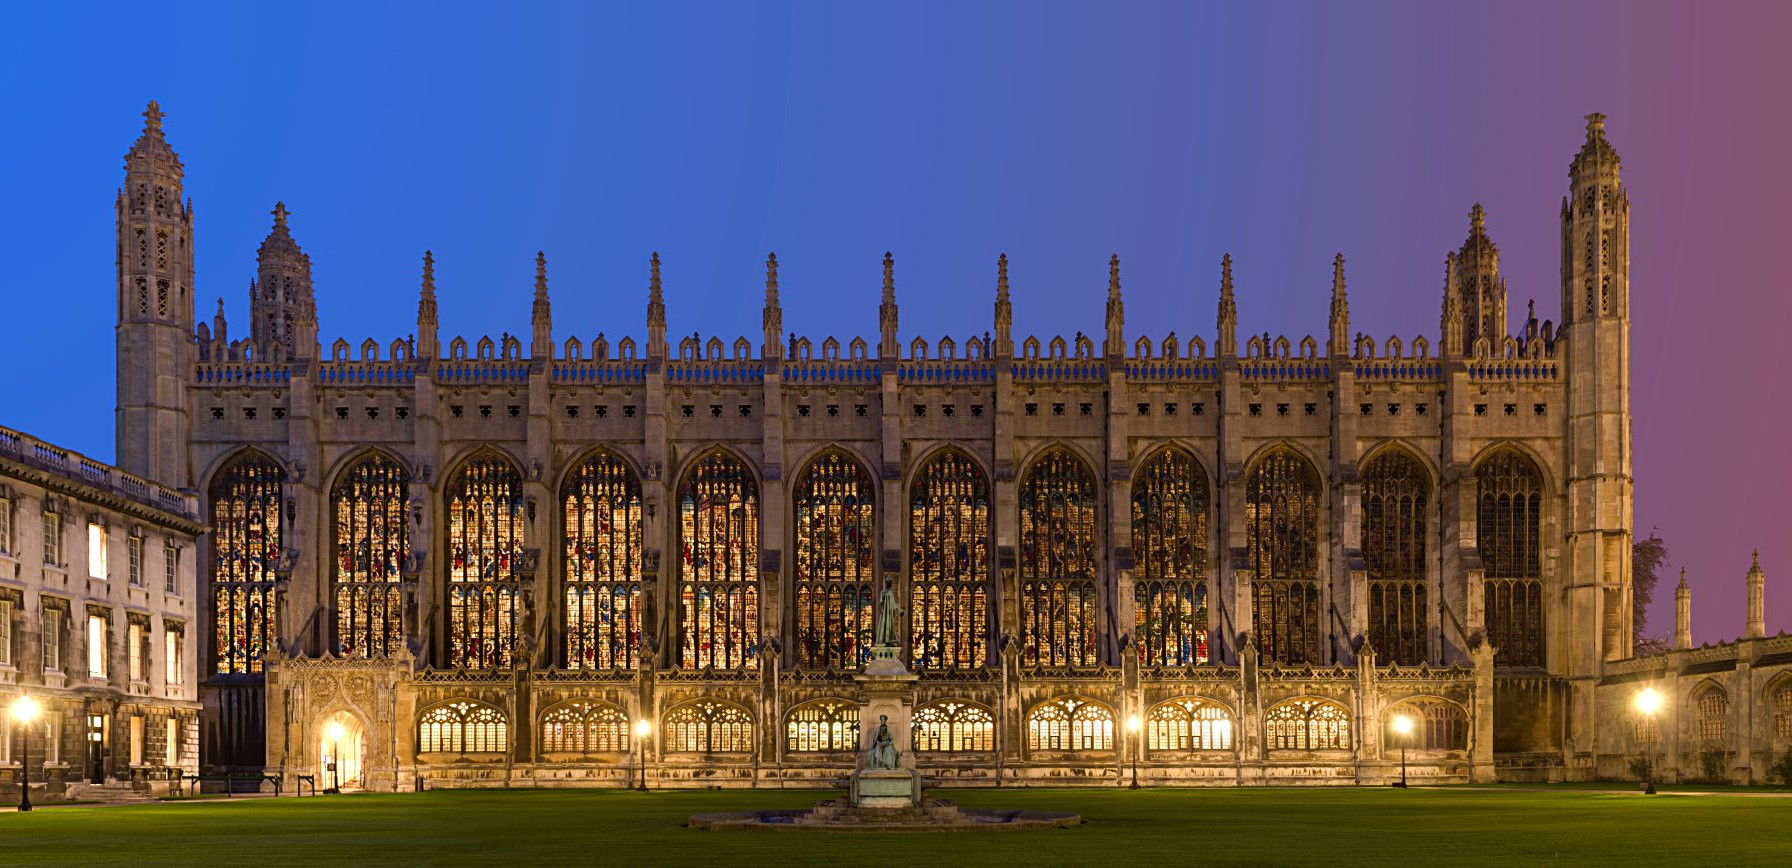
\includegraphics[width=\textwidth]{figs/kings.jpg}
	\end{figure}
\end{frame}


%------------------------------------------------
\begin{frame}
	\frametitle{\faQuestionCircleO~What is the thickness of the ceiling?}
	\begin{figure}[ht]
		\centering
		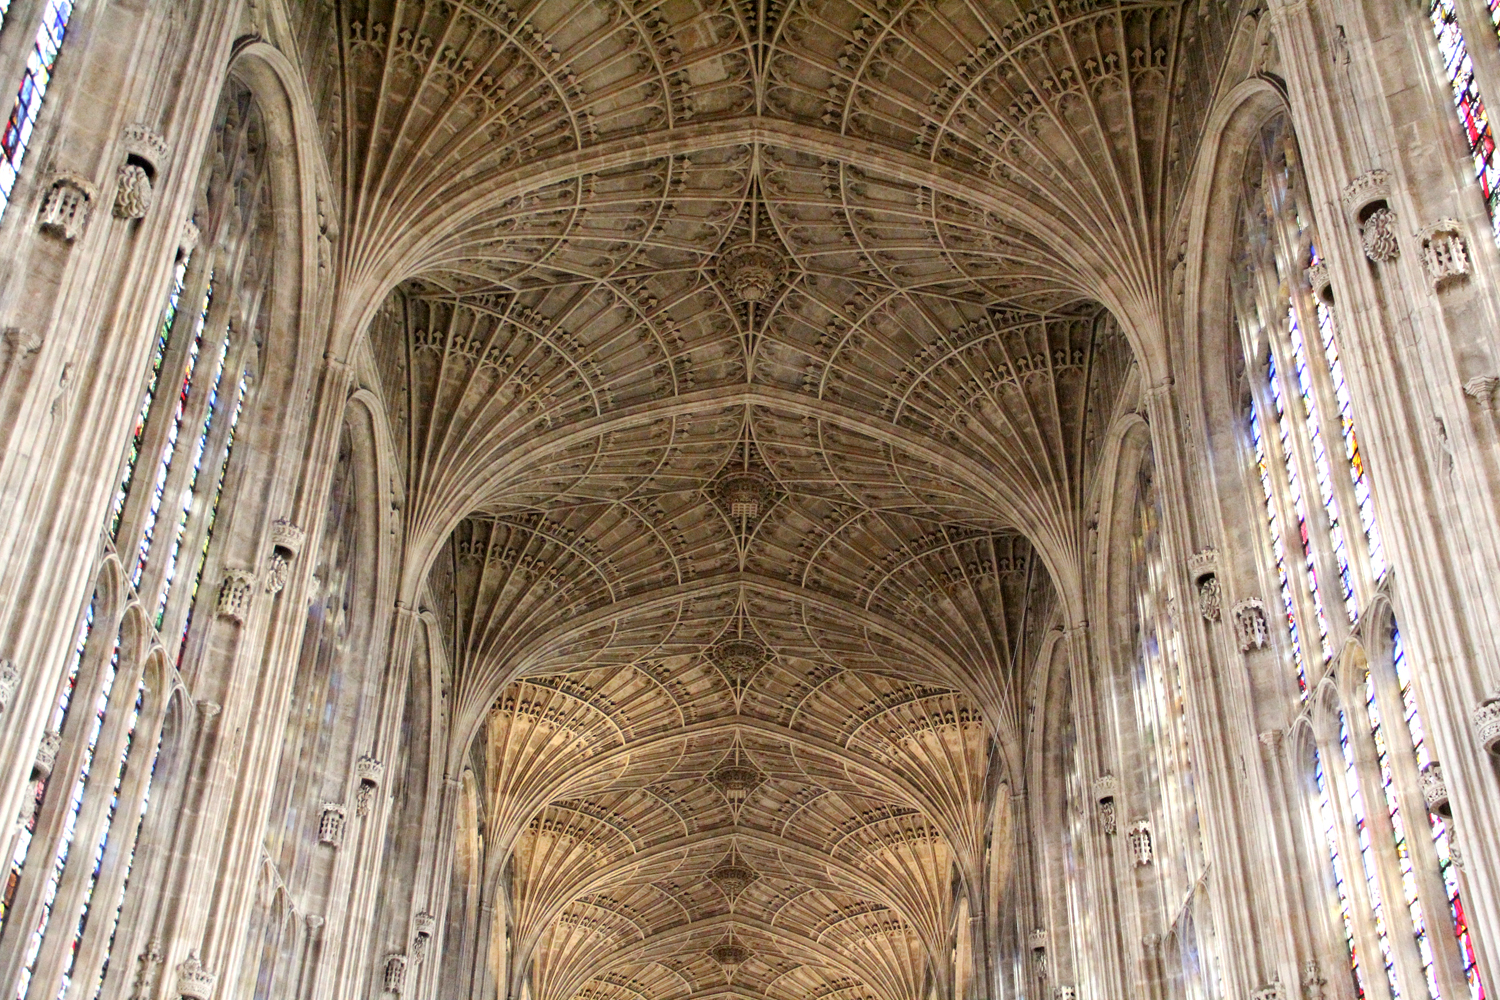
\includegraphics[width=0.8\textwidth]{figs/fanvaults.jpg}
	\end{figure}
\end{frame}

%------------------------------------------------
\begin{frame}
	\frametitle{From arches to fan vaults}
	\begin{figure}[ht]
		\centering
		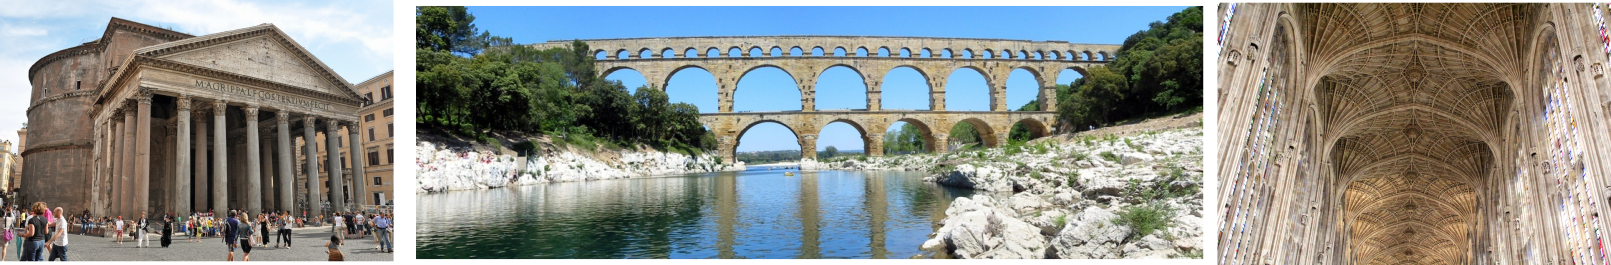
\includegraphics[width=\textwidth]{figs/arches-fan-vaults.png}
	\end{figure}
\end{frame}

%------------------------------------------------
\begin{frame}
	\frametitle{The fan vaults of King's college}
	\begin{figure}[ht]
		\centering
		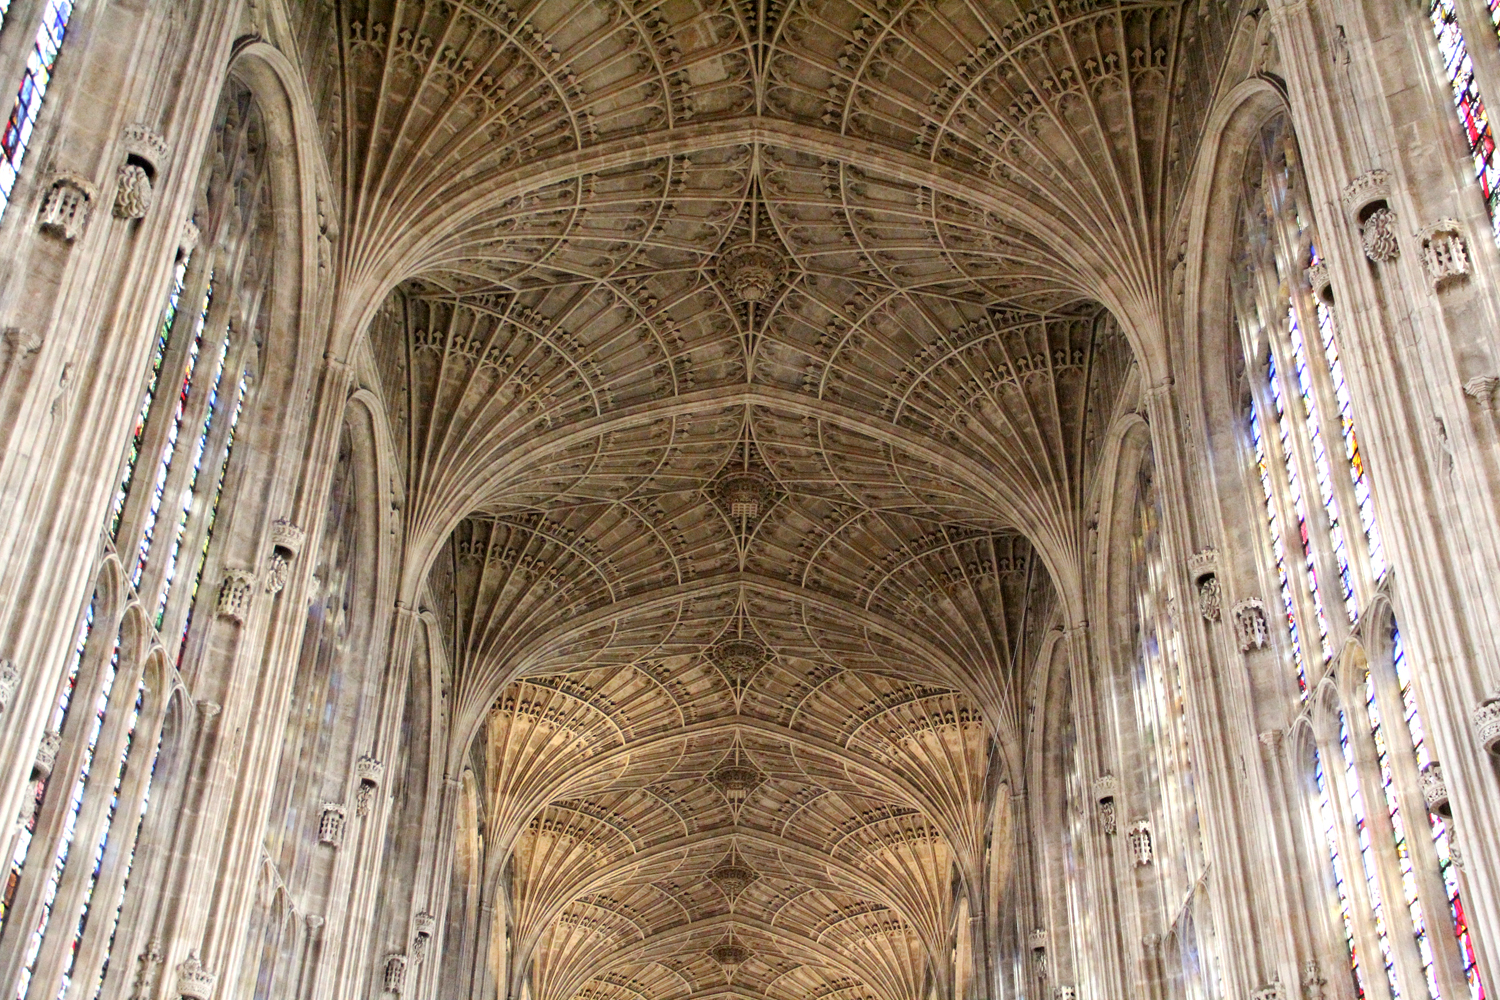
\includegraphics[width=0.8\textwidth]{figs/fanvaults.jpg}
	\end{figure}
\end{frame}

\note{King's college fan vaults were built in 1500s}

%------------------------------------------------
\begin{frame}
	\frametitle{Catenary}
	\begin{figure}[ht]
		\centering
		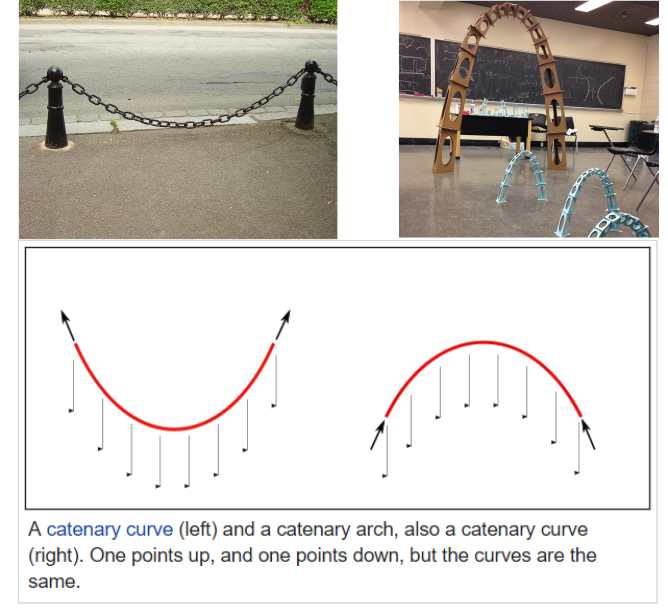
\includegraphics[width=0.65\textwidth]{figs/catenary.png}
	\end{figure}
\end{frame}

\note{The English architect Robert Hooke was the first to study the 
	catenary mathematically and in 1675 published an anagram (in Latin) 
	of : "As hangs the flexible line, so but inverted will stand the 
	rigid arch." The arch above Wembley Stadium has the shape of a 
	catenary and Christopher Wren also intended to use it in St. 
	Paul's dome }

%------------------------------------------------
\begin{frame}
	\frametitle{Sagrada Familia}
	\begin{figure}[ht]
		\centering
		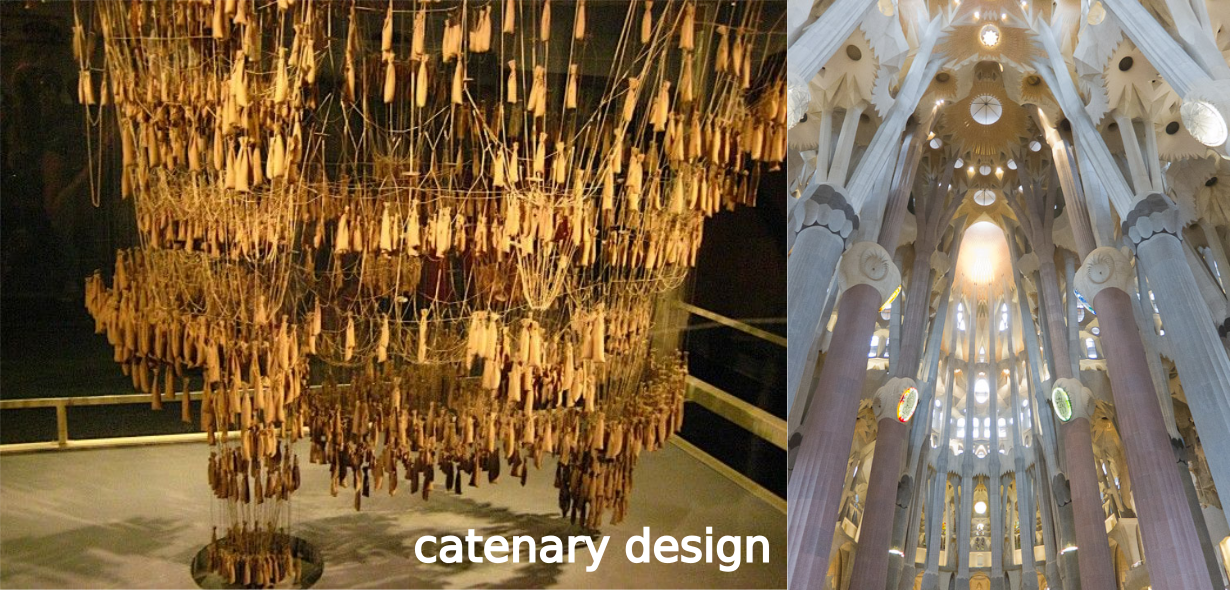
\includegraphics[width=\textwidth]{figs/sagrada-familia.png}
	\end{figure}
\end{frame}

\note{Antoni Gaudi i Cornet (1852-1926) was a well-known architect from Spain.
	Gaudi used catenary arches in many of his projects. One of Gaudi's greatest works however became the Temple of the Holy Family (the Sagrada Familia) in Barcelona.}

%------------------------------------------------
\begin{frame}
	\frametitle{Catenary, caternary \dots everywhere}
	\begin{figure}[ht]
		\centering
		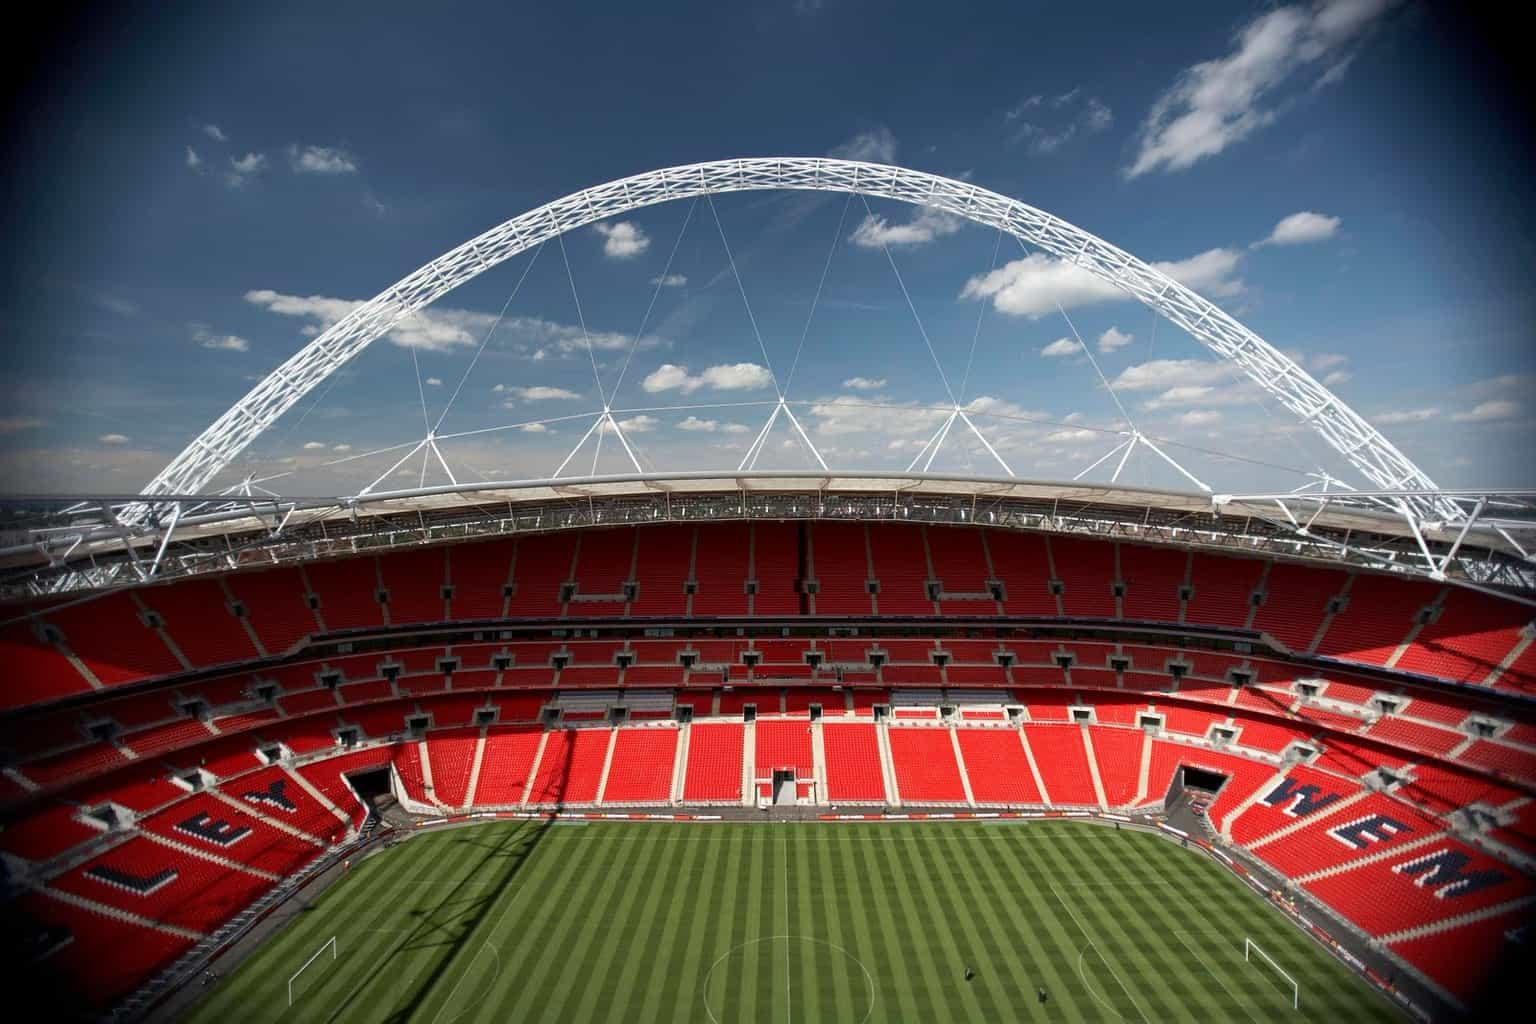
\includegraphics[width=0.95\textwidth]{figs/wembley.jpg}
	\end{figure}
\end{frame}

%------------------------------------------------
\begin{frame}
	\frametitle{\faQuestionCircleO ~What is this shape?}
	\begin{figure}[ht]
		\centering
		\includegraphics[width=\textwidth]{figs/parabola.jpg}
	\end{figure}
\end{frame}


%------------------------------------------------
\begin{frame}
	\frametitle{Catenary vs Parabola}
	\begin{figure}[ht]
		\centering
		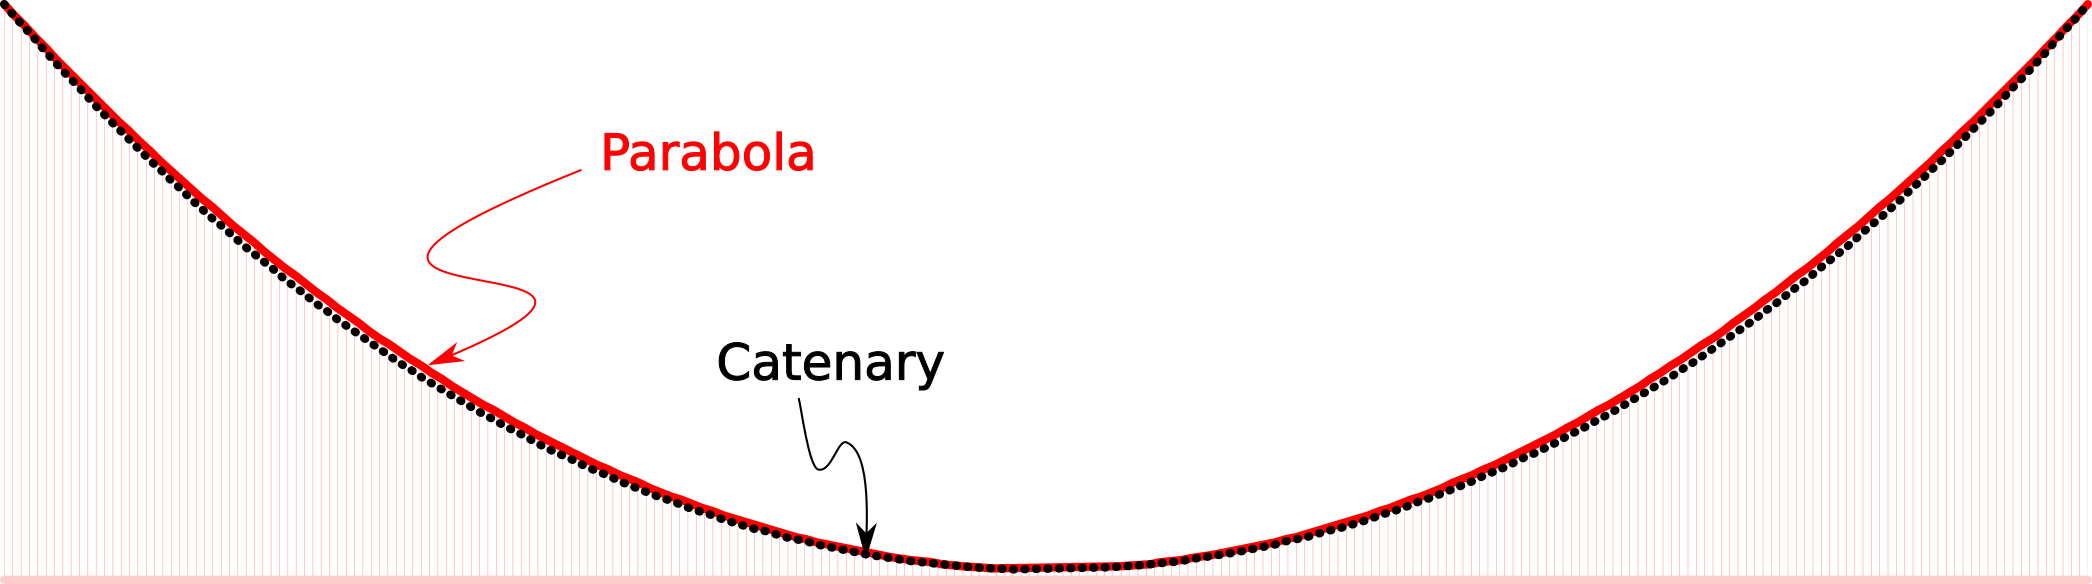
\includegraphics[width=\textwidth]{figs/catenary_parabola.png}
	\end{figure}
\end{frame}

\note{Parabola $y = x^2$ for a parabola, a hyperbolic function like $\cosh(x)\approx = 1 + \frac{x^2}{2}$}

%------------------------------------------------
\begin{frame}
	\frametitle{Potential energy of a simple pendulum}
	We need to know how high the weight of the pendulum is above its lowest point
	\begin{figure}[ht]
		\centering
		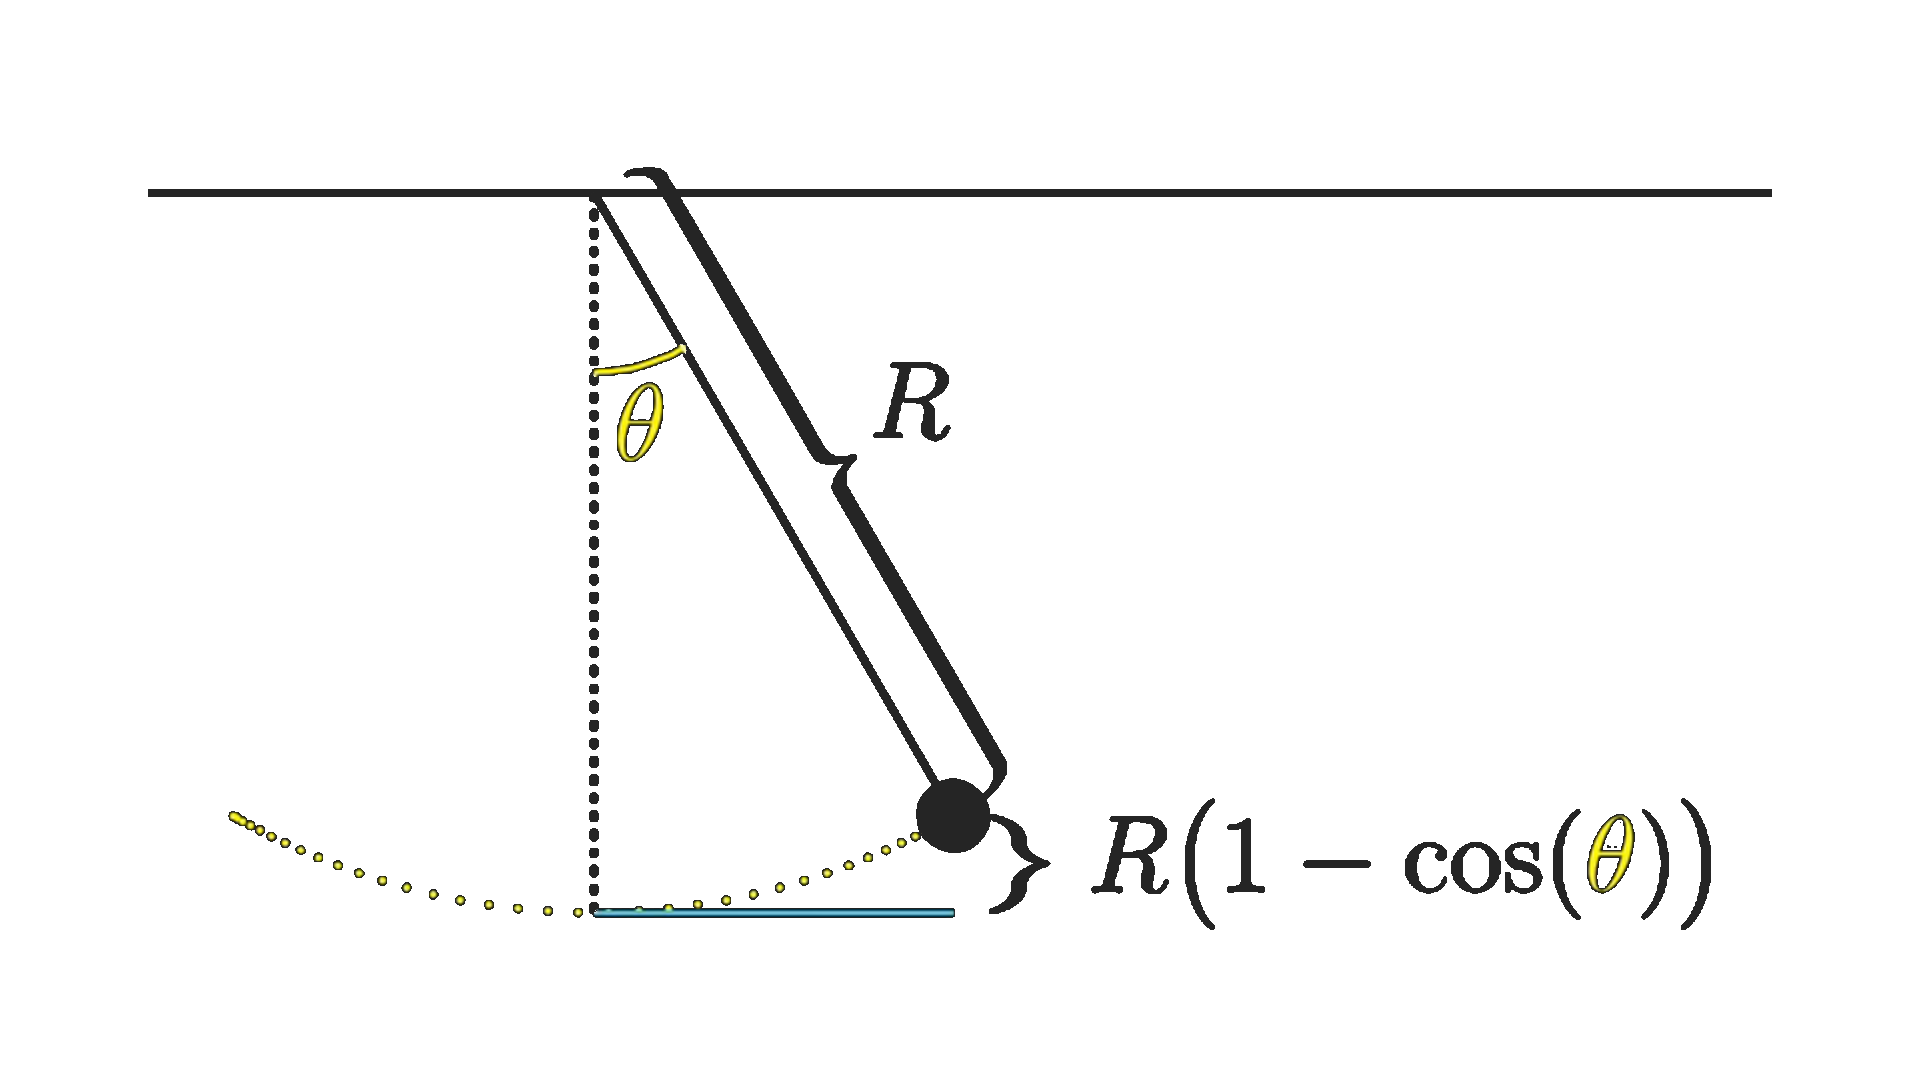
\includegraphics[width=\textwidth]{figs/simple-pendulum.png}
	\end{figure}
\end{frame}


\note{Taylor series approximation $\cos(\theta) \approx $ for a parabola, a hyperbolic 
	function like $\cosh(x)\approx 1 + \frac{x^2}{2}$, which gives 
	$h = R(1 - (1 + \frac{\theta^2}{2})) = R \frac{\theta^2}{2}$

The cosine function made the problem awkward and unweildy. If we approximate using 
$\cos(\theta) \approx \frac{\theta^2}{2}$ everything fell into place. An approximation 
like that might seem completely out of left field. Let's graph these functions. They do 
look close to each other. But how do we think to make this approximation? and how do we even get that particular quadratic?
}

\section{Taylor series}
%------------------------------------------------
\begin{frame}
	\frametitle{Taylor series}
	\mode<beamer>{
		\begin{itemize}
			\item Taylor series is one the best tools maths has to offer for approximating functions. 
			
			\item Taylor series is about taking non-polynomial functions and finding polyomials that approximate at some input. 
			
			\item The motive here is the polynomials tend to be much easier to deal with than other functions, they are easier to compute, take derivatives, integrate, just easier overall. 
			
			\item $e^x = 1 + x + \frac{x^2}{2!} + \frac{x^3}{3!} + \dots$
		\end{itemize}
	}
	\mode<handout>{
		\vspace{5cm}
	}
\end{frame}


%------------------------------------------------
\begin{frame}
	\frametitle{Taylor series of cos(x)}
	\begin{figure}[ht]
		\centering
		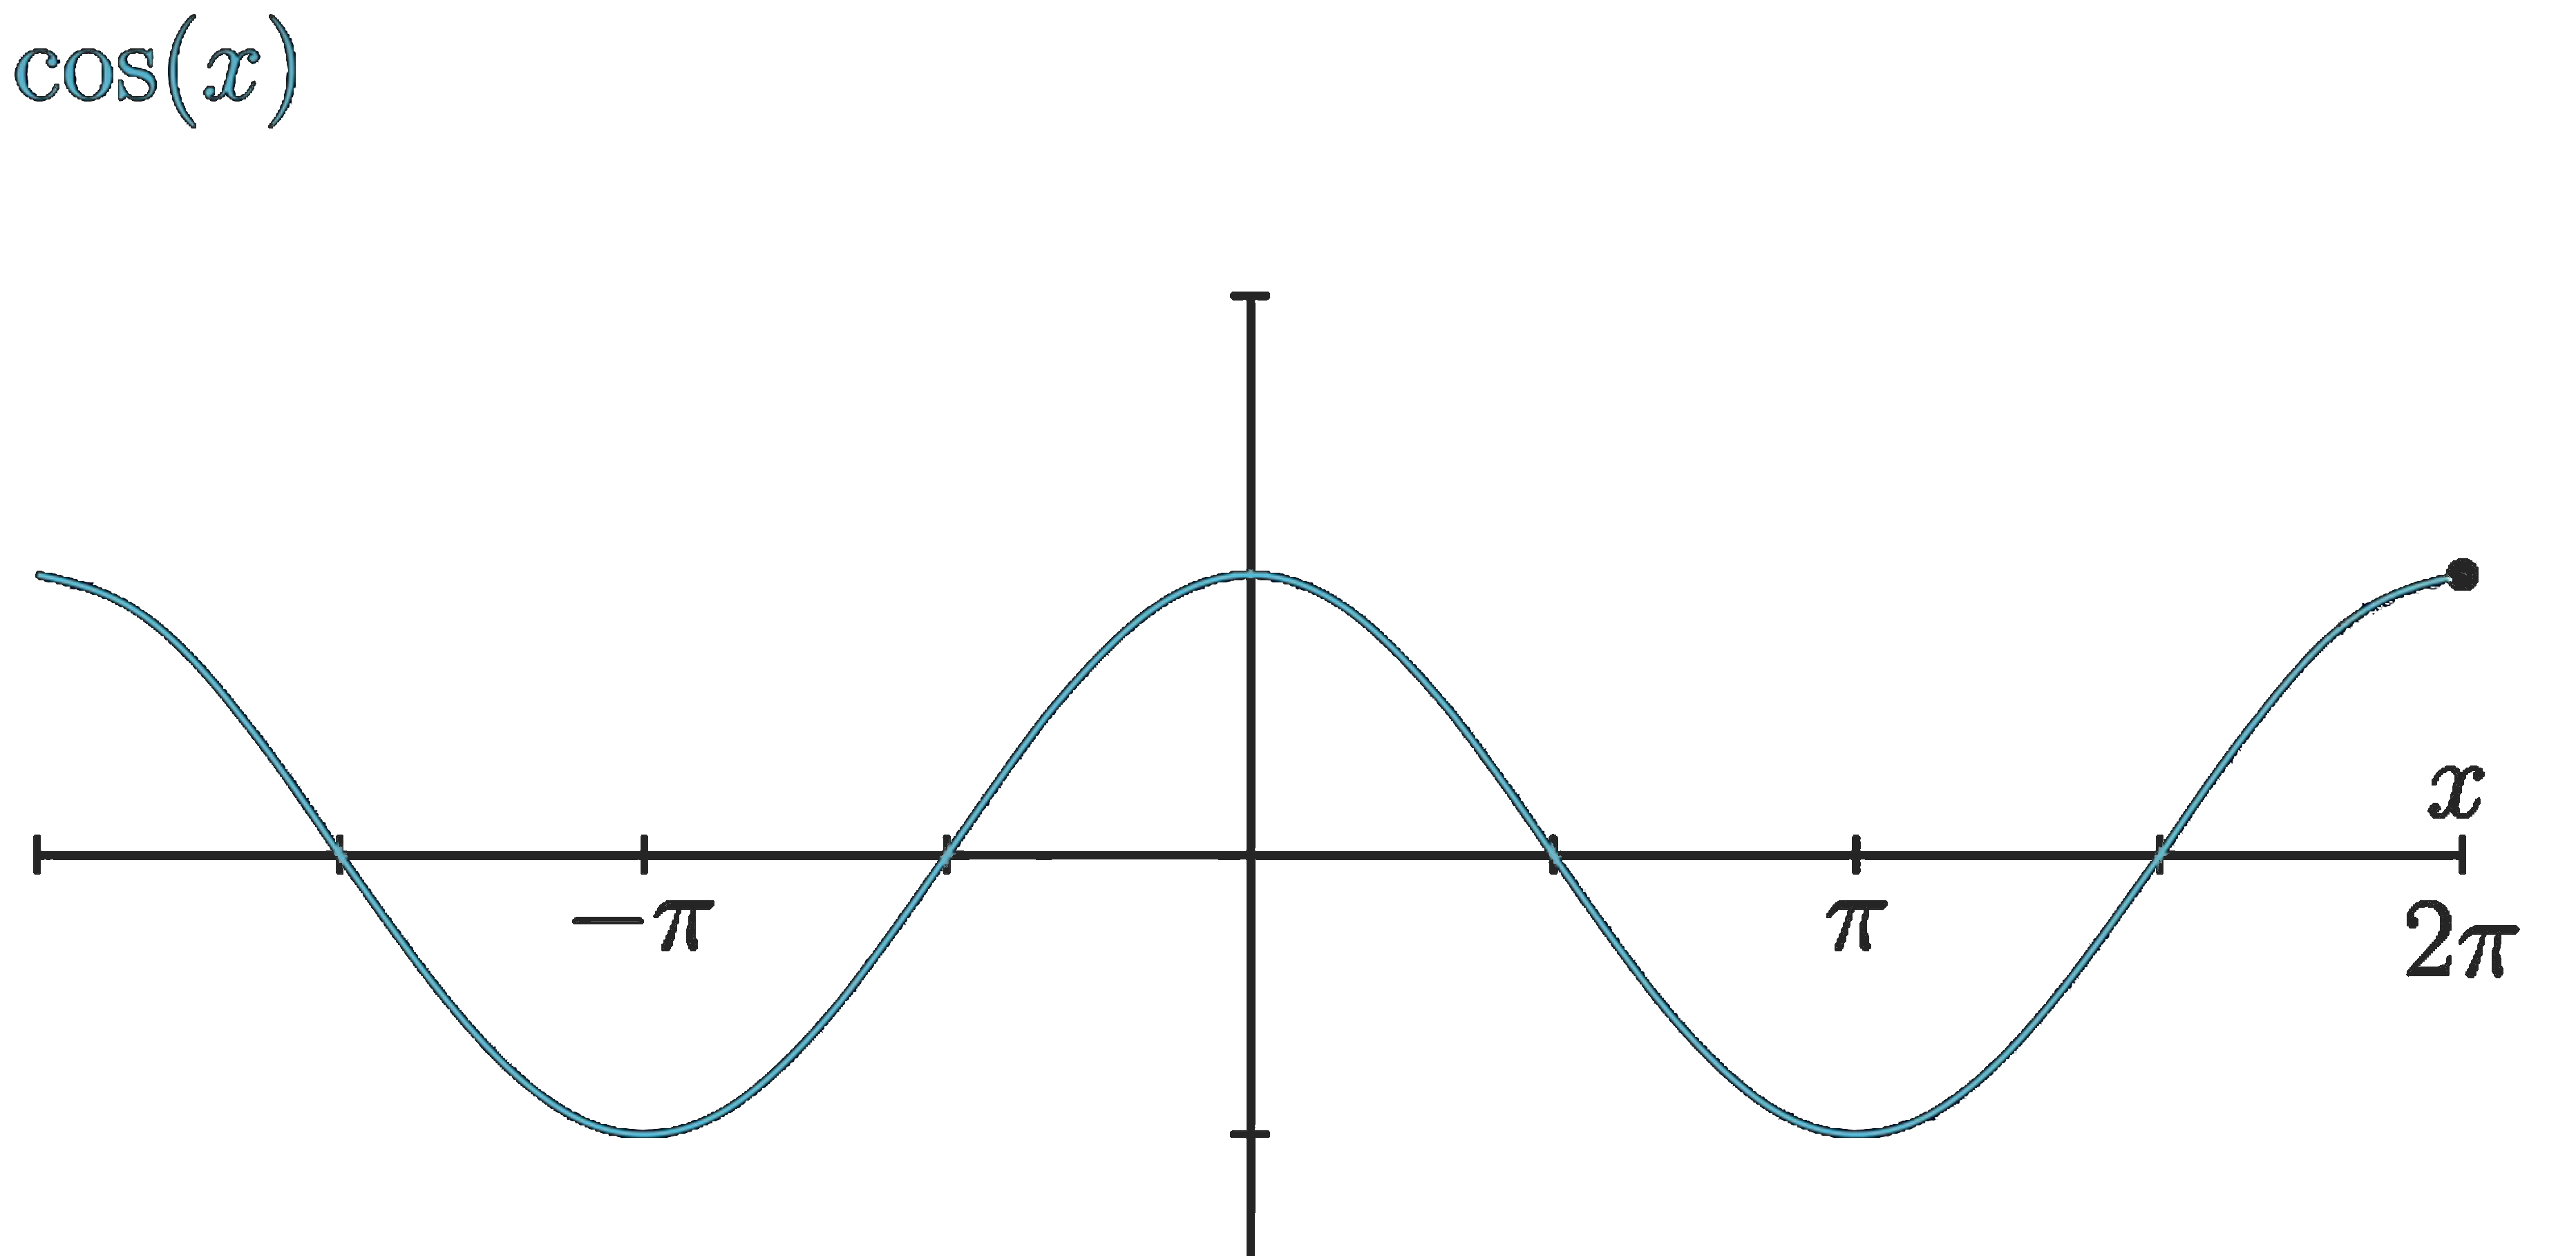
\includegraphics[width=\textwidth]{figs/cosx.png}
	\end{figure}
\end{frame}


%------------------------------------------------
\begin{frame}
	\frametitle{Taylor series of cos(x)}
	\begin{figure}[ht]
		\centering
		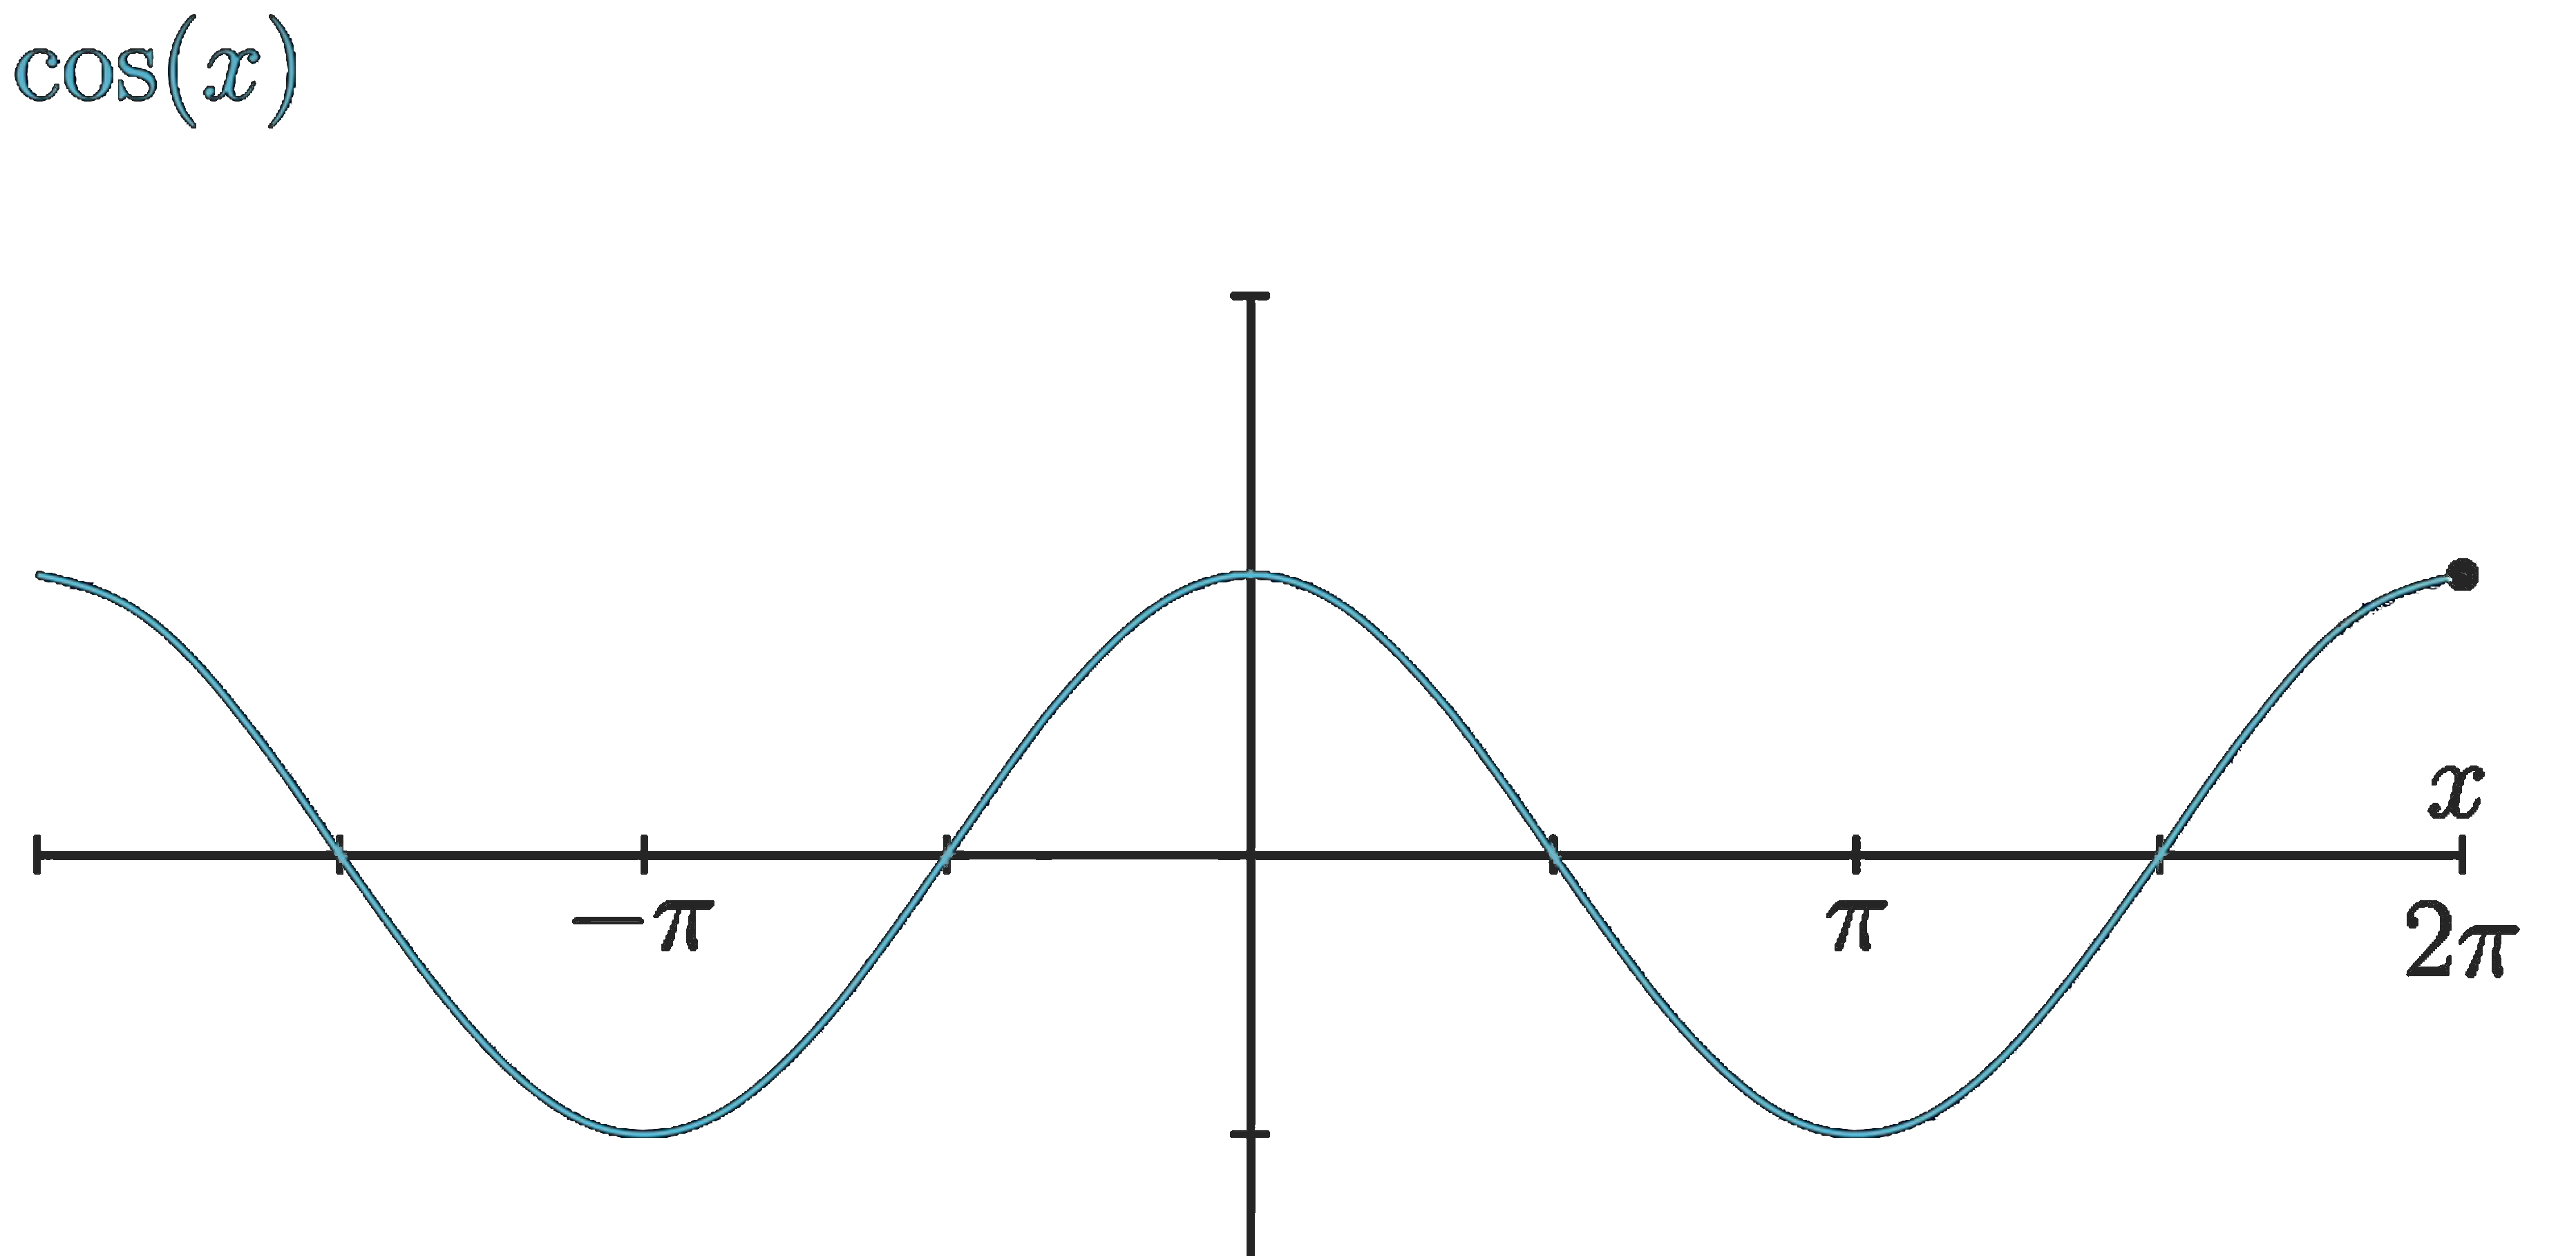
\includegraphics[width=\textwidth]{figs/cosx.png}
	\end{figure}
\end{frame}


%------------------------------------------------
\begin{frame}
	\frametitle{Taylor series of cos(x)}
	\mode<beamer>{
		\begin{figure}[ht]
			\centering
			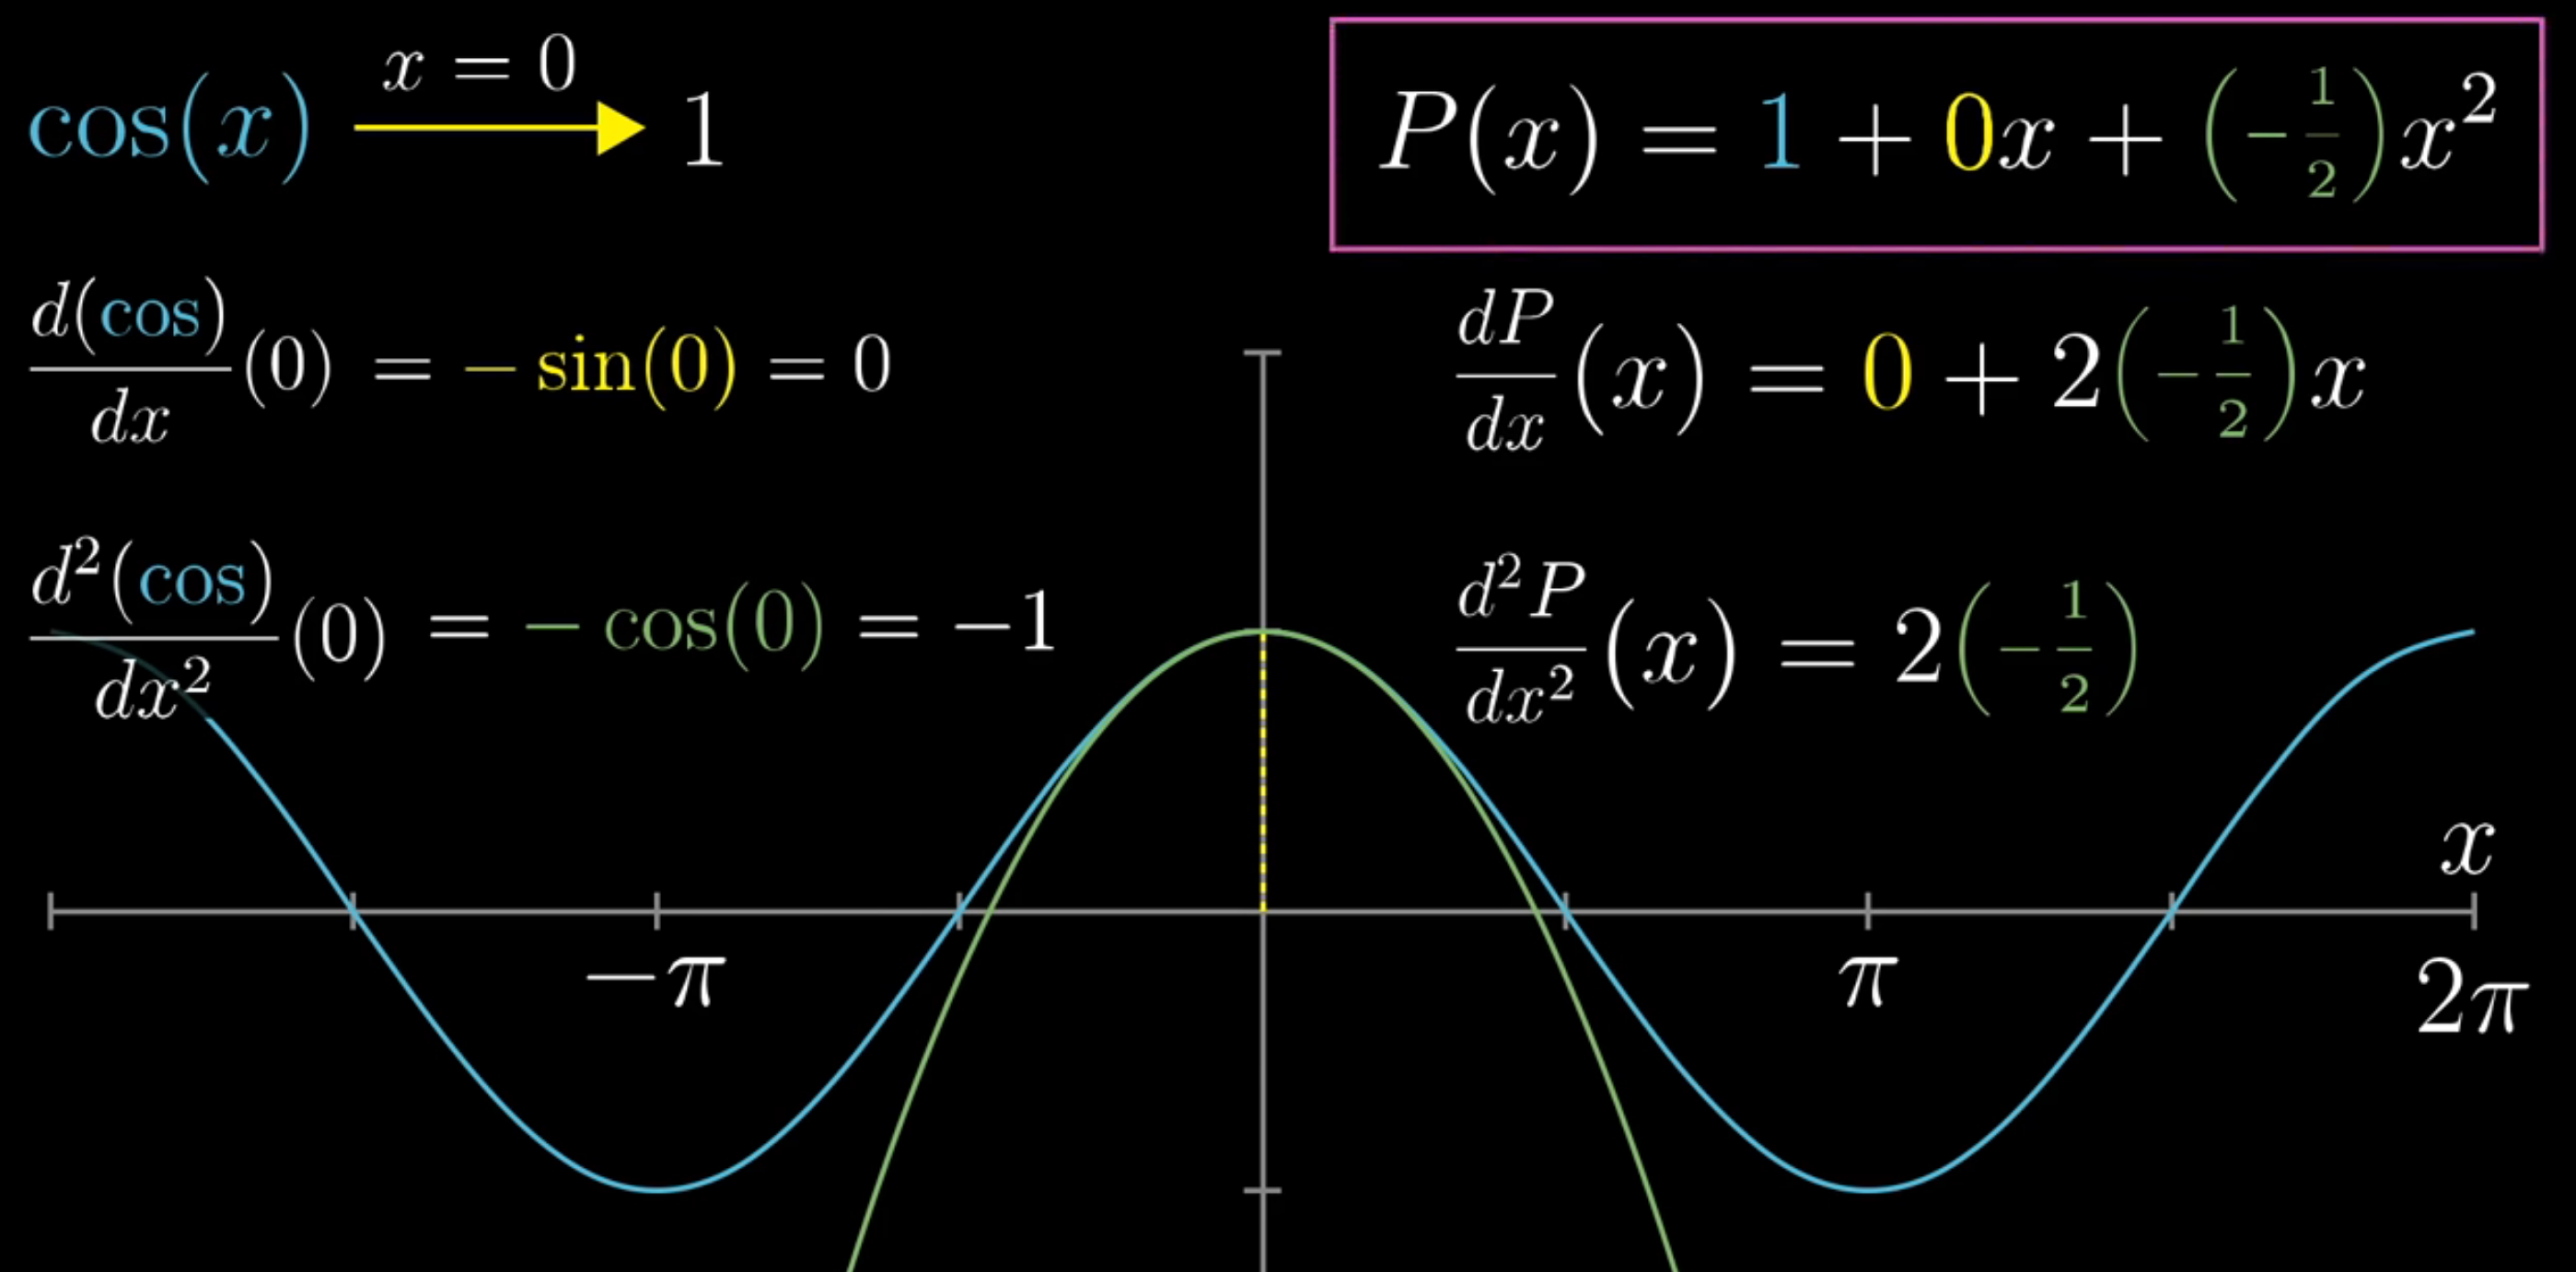
\includegraphics[width=\textwidth]{figs/cosx_approx.png}
		\end{figure}
	}
	\mode<handout>{
	\begin{figure}[ht]
		\centering
		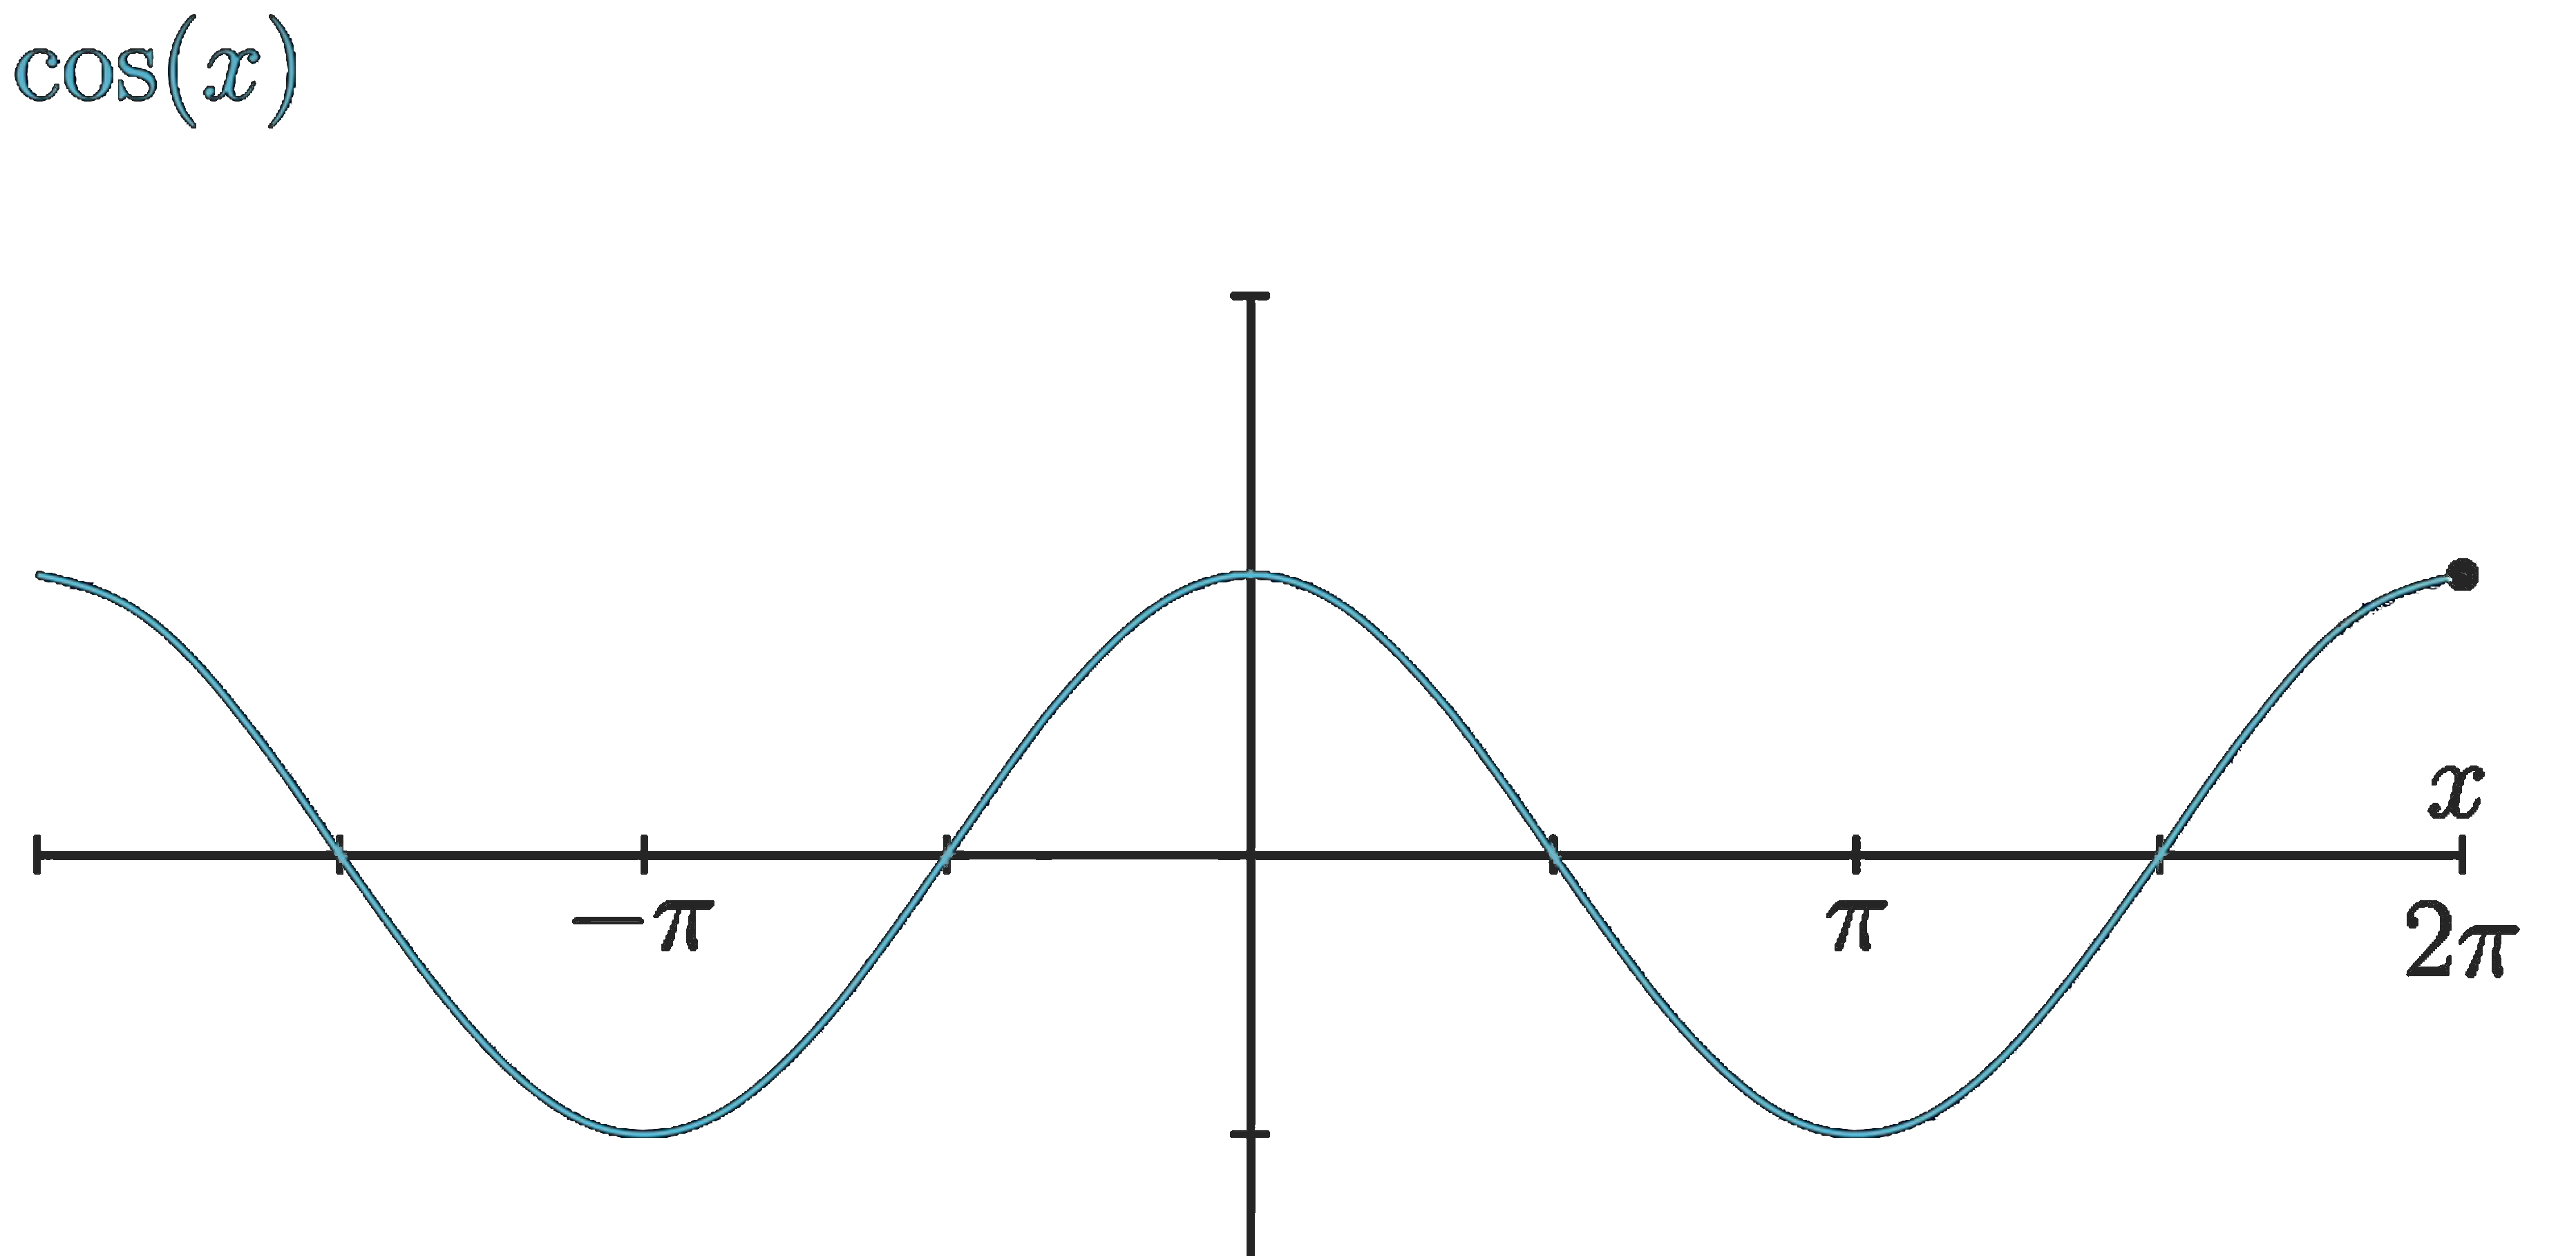
\includegraphics[width=\textwidth]{figs/cosx.png}
	\end{figure}
	}
\end{frame}



%------------------------------------------------
\begin{frame}
	\frametitle{Taylor series of cos(x): 4th derivative}
	\mode<beamer>{
	\begin{align*}
		P(x) & = 1 - \frac{1}{2}x^2 + \frac{1}{24}x^4 \\
		\frac{d^4P}{dx^4}(x) & = 1\cdot 2 \cdot 3 \cdot 4 \cdot \frac{1}{24}\\
		& = 24 \cdot \frac{1}{24}
	\end{align*}
	
	To find the coefficient of $n^{th}$ term:
	
	\begin{align*}
		\frac{d^8}{dx^8}(c_8x^8) & = 1\cdot 2\cdot 3\cdot 4\cdot 5\cdot 6\cdot 7\cdot 8\cdot c_8\\
		& = 8! \\
		Set~ c_8& = \frac{\mathrm{desired~ derivative~ value}}{8!}
	\end{align*} 
	}
	\mode<handout>{
		\begin{figure}[ht]
			\centering
			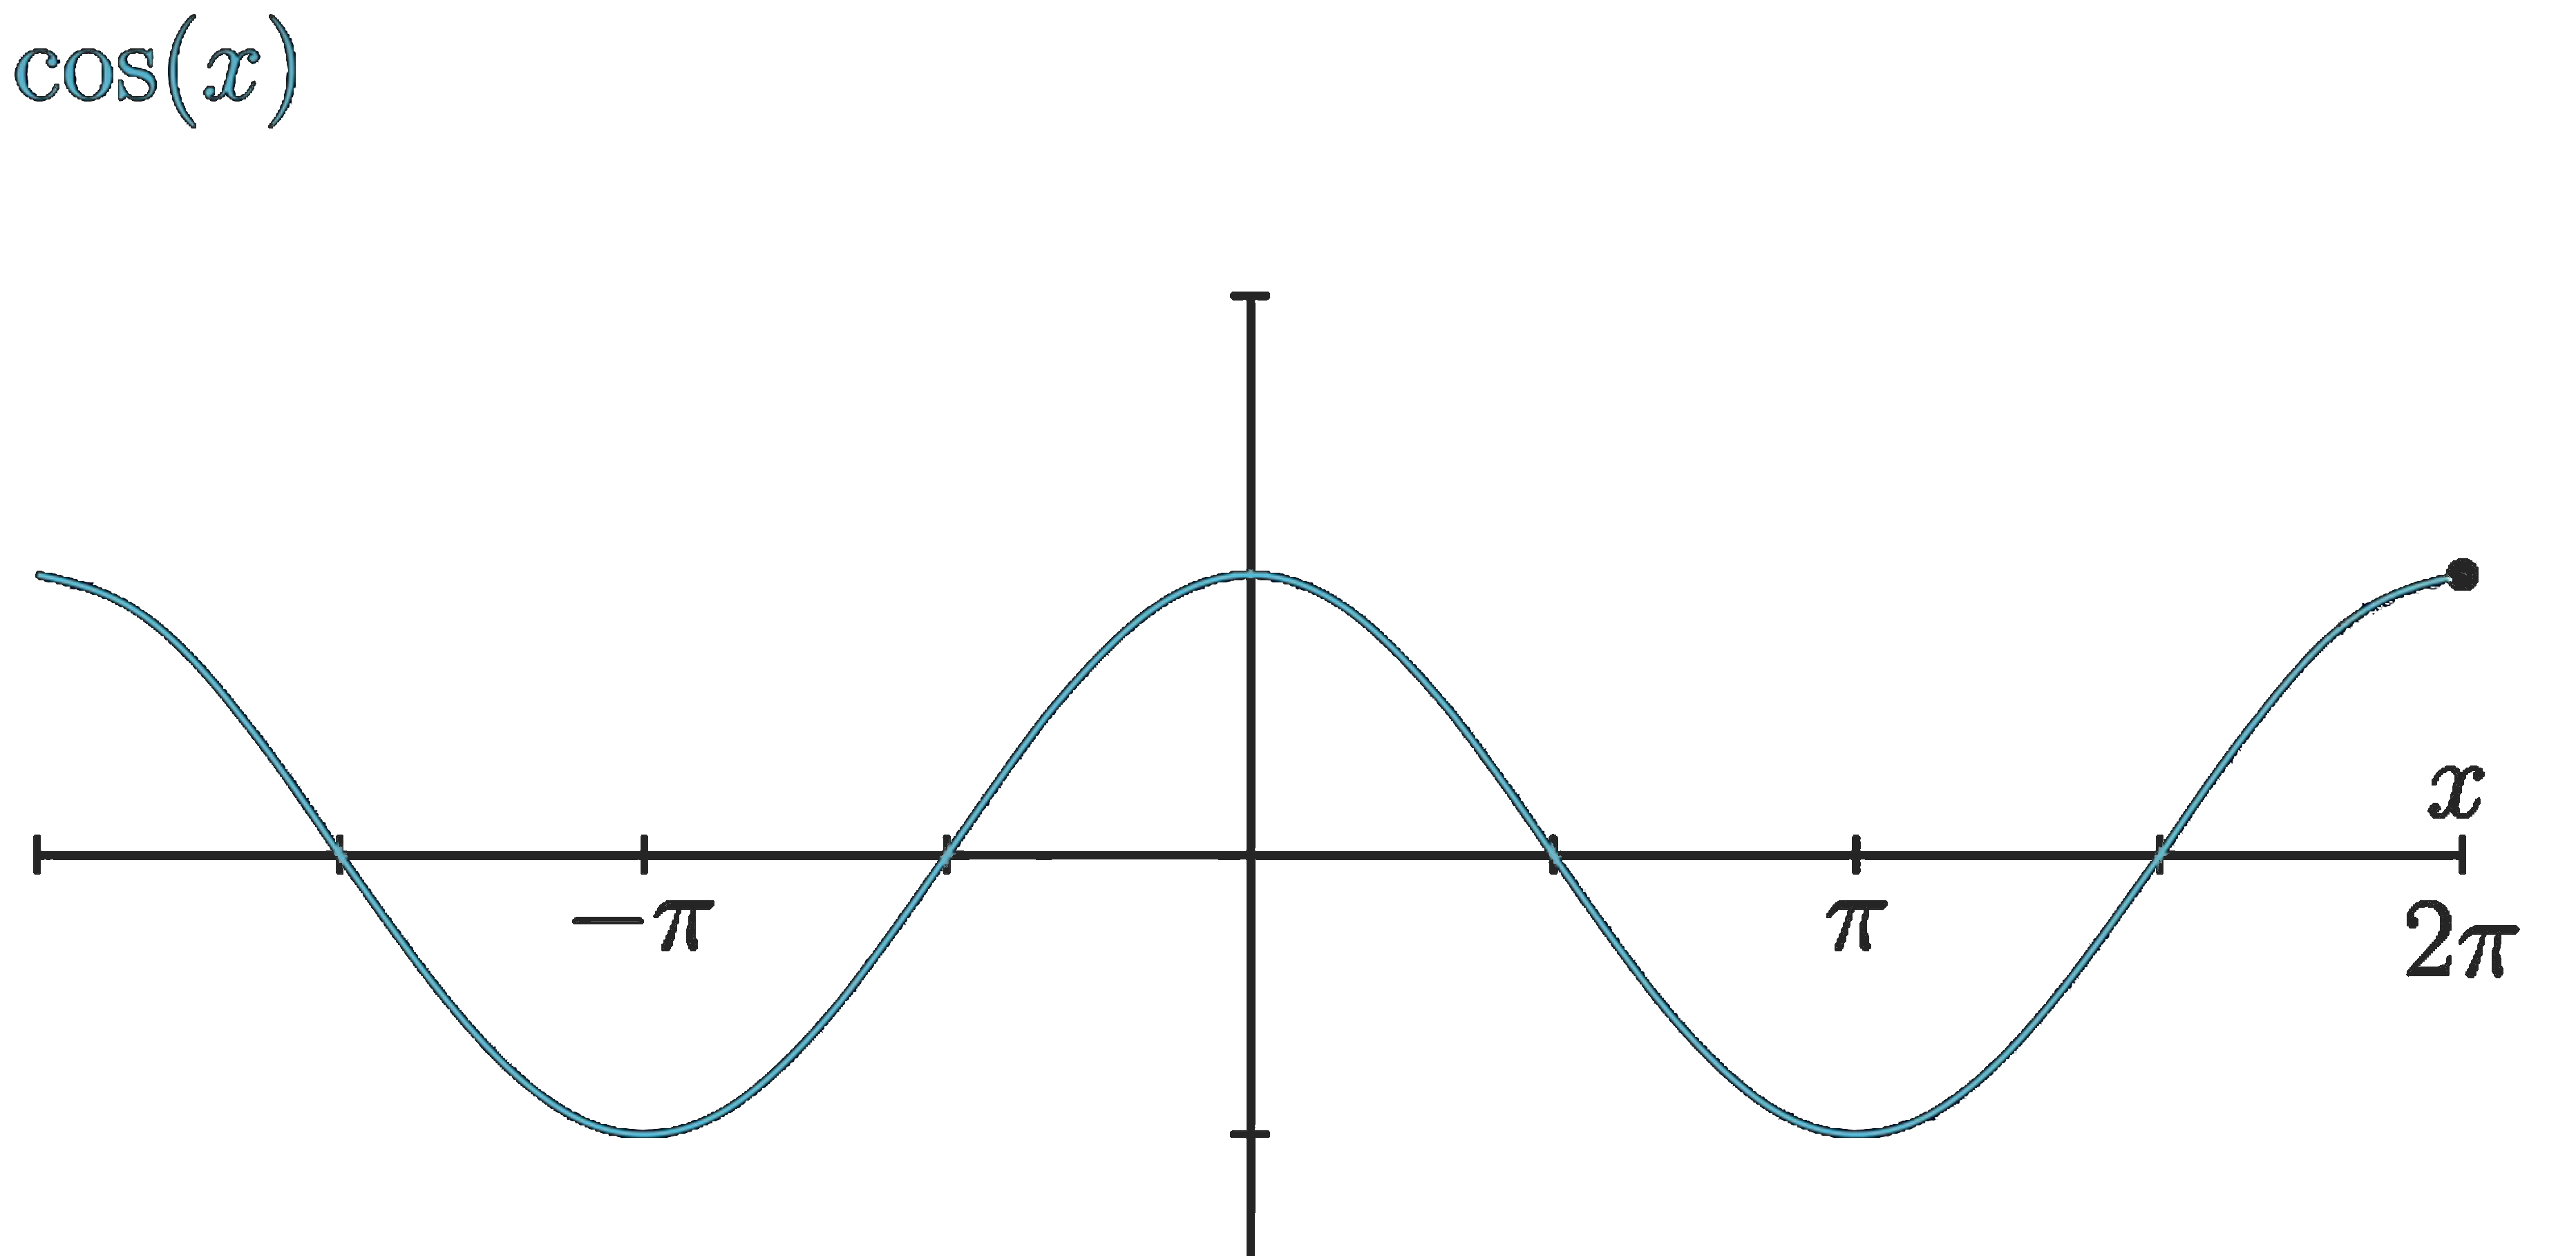
\includegraphics[width=\textwidth]{figs/cosx.png}
		\end{figure}
	}
\end{frame}

%------------------------------------------------
\begin{frame}
	\frametitle{Taylor series of cos(x)}
	\mode<beamer>{
		\begin{figure}[ht]
			\centering
			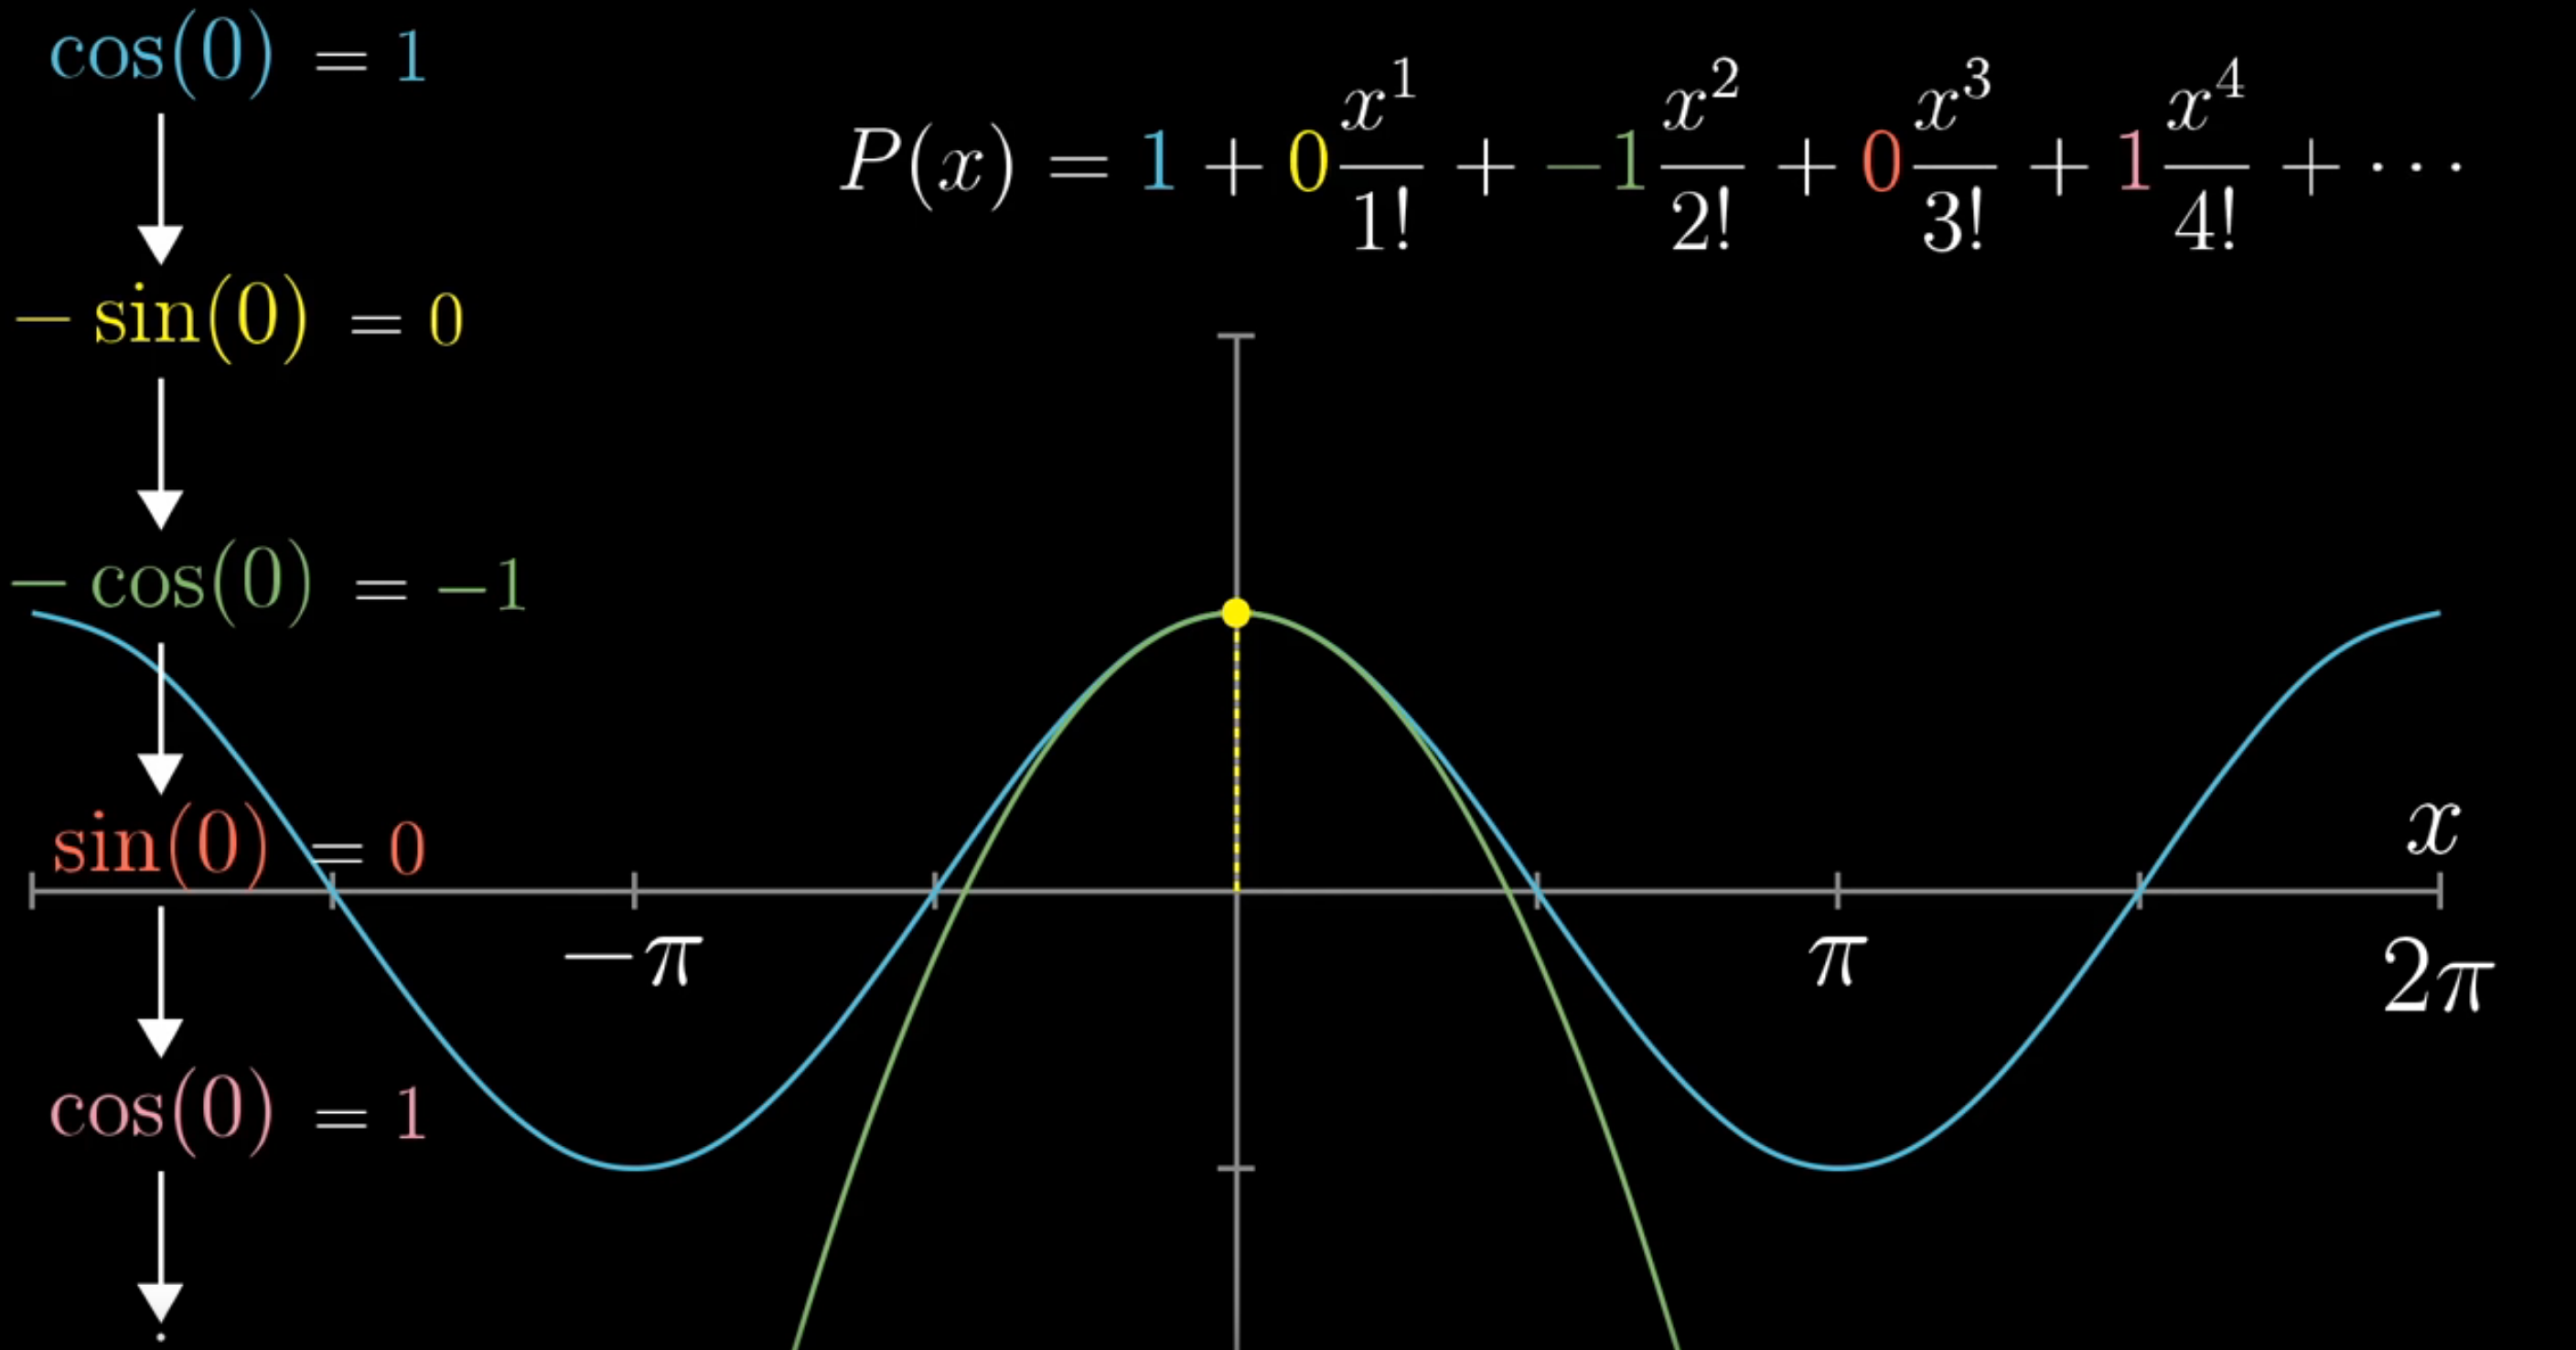
\includegraphics[width=\textwidth]{figs/cos_coefficients.png}
		\end{figure}
	}
	\mode<handout>{
		\vspace{5cm}
	}
\end{frame}

%------------------------------------------------
\begin{frame}
	\frametitle{Taylor series: Generalization}
	\mode<beamer>{
		\begin{figure}[ht]
			\centering
			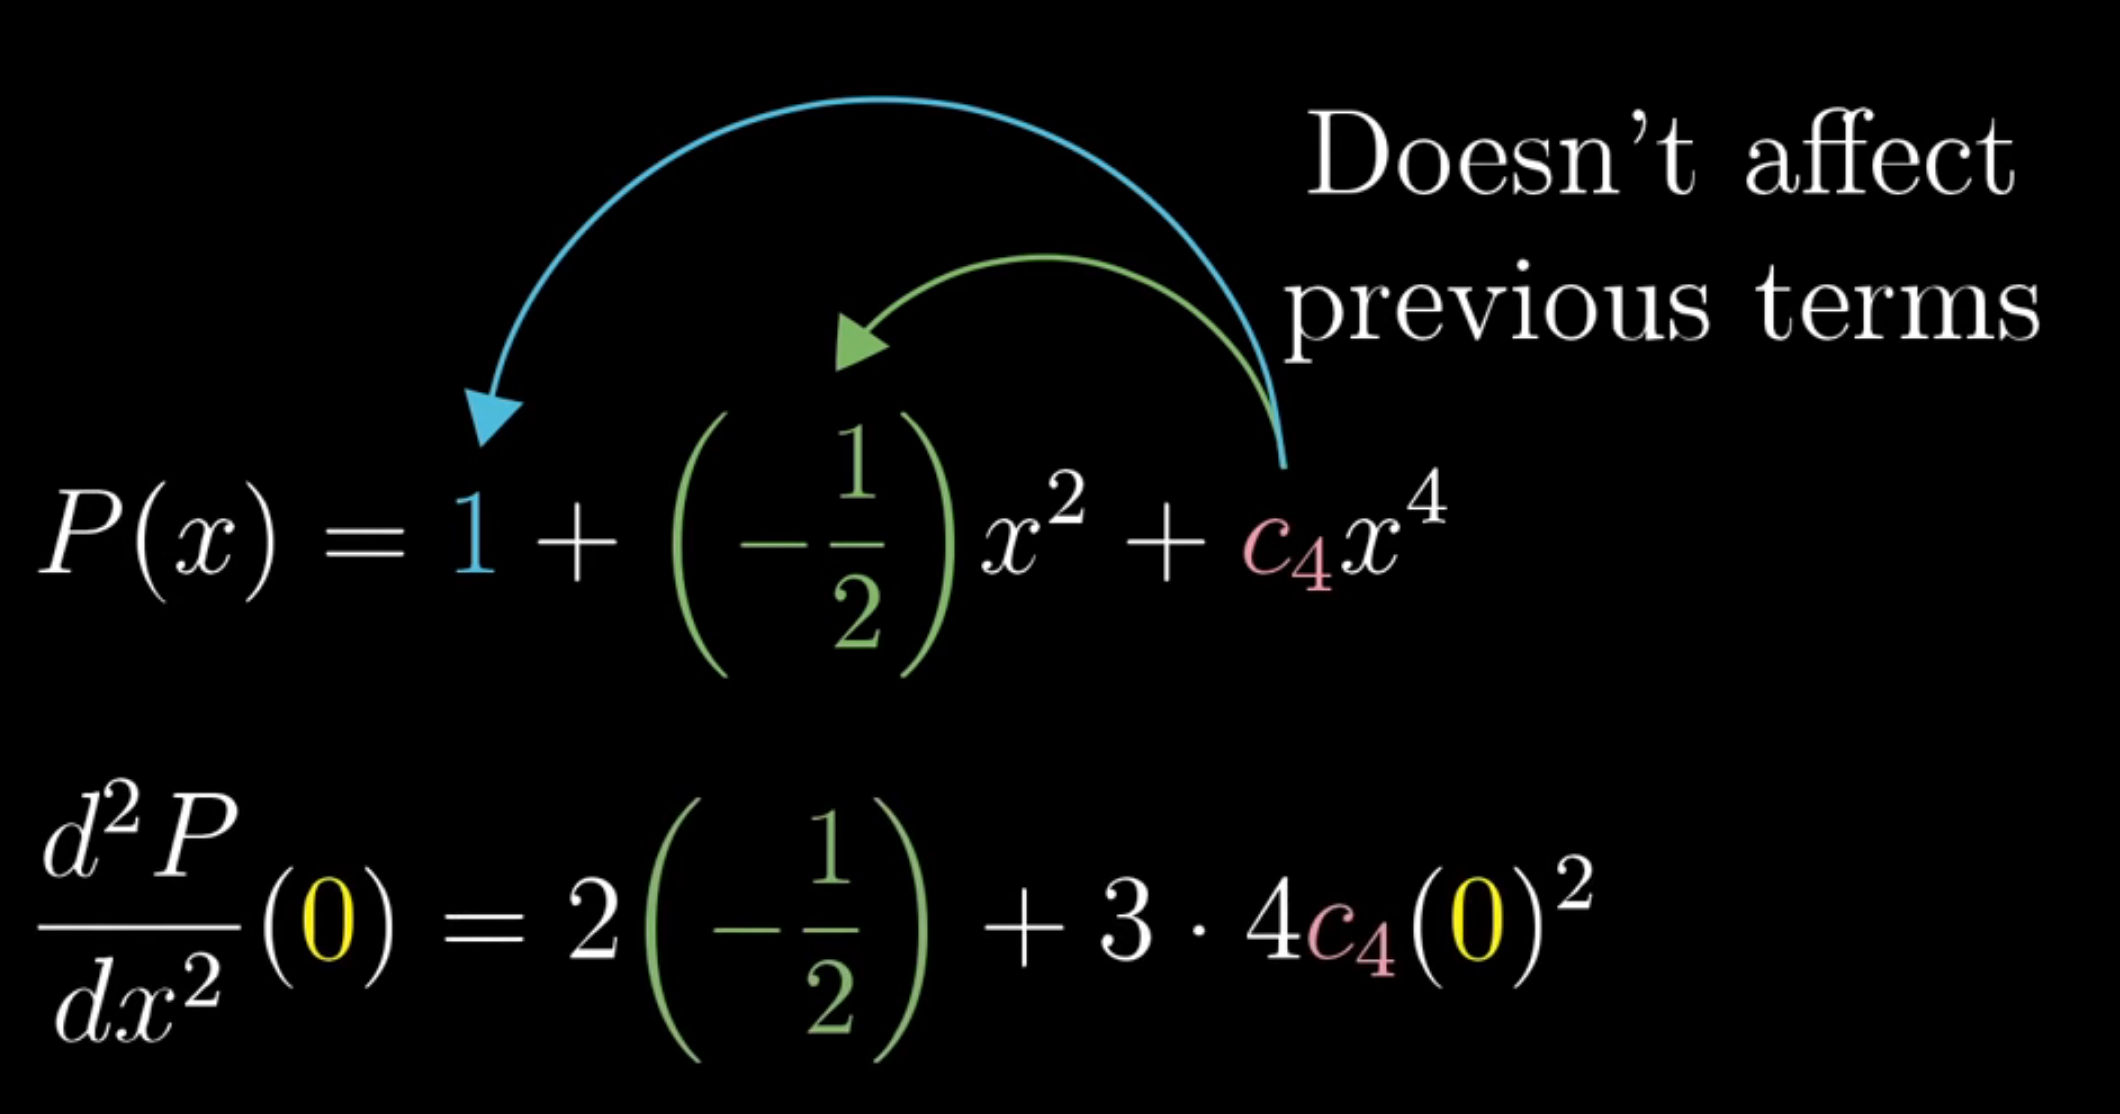
\includegraphics[width=0.6\textwidth]{figs/taylor-series.png}
		\end{figure}
		\begin{figure}[ht]
			\centering
			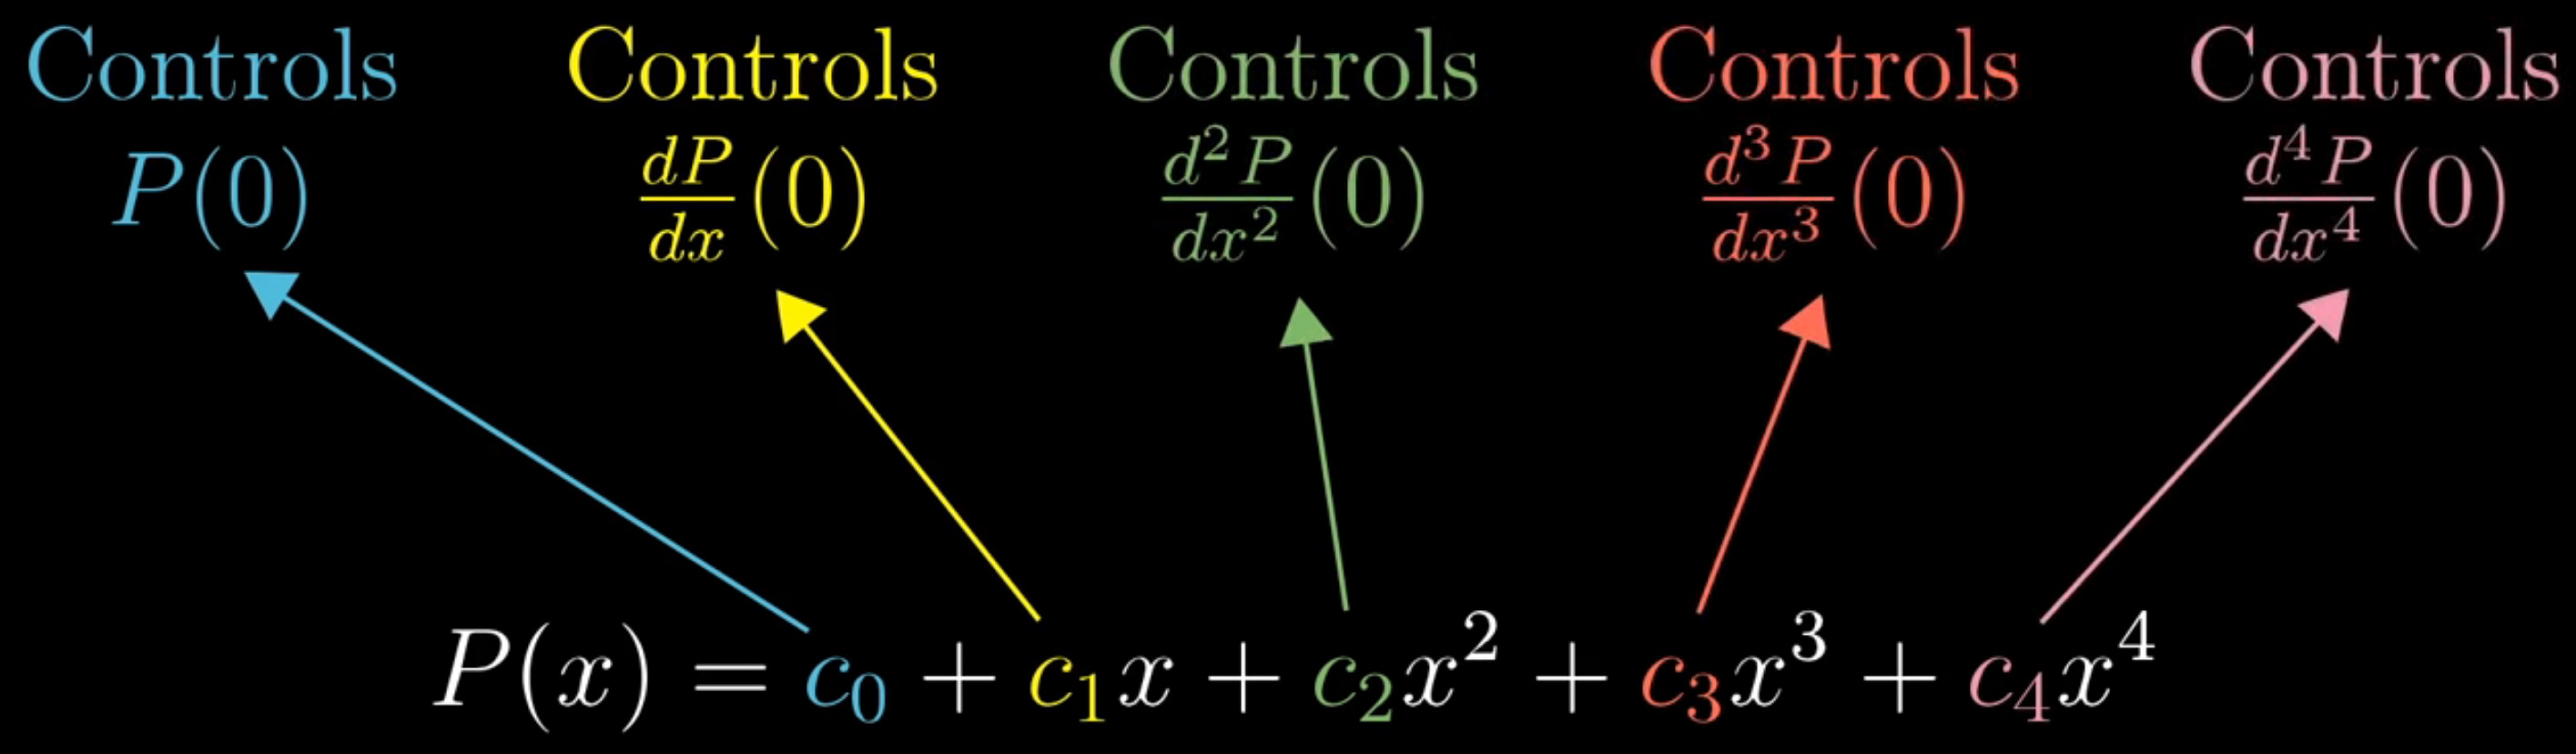
\includegraphics[width=0.6\textwidth]{figs/taylor-terms.png}
		\end{figure}
	}
	\mode<handout>{
		\vspace{5cm}
	}
\end{frame}

%------------------------------------------------
\begin{frame}
	\frametitle{Taylor series: Generalization}
	\mode<beamer>{
		\begin{figure}[ht]
			\centering
			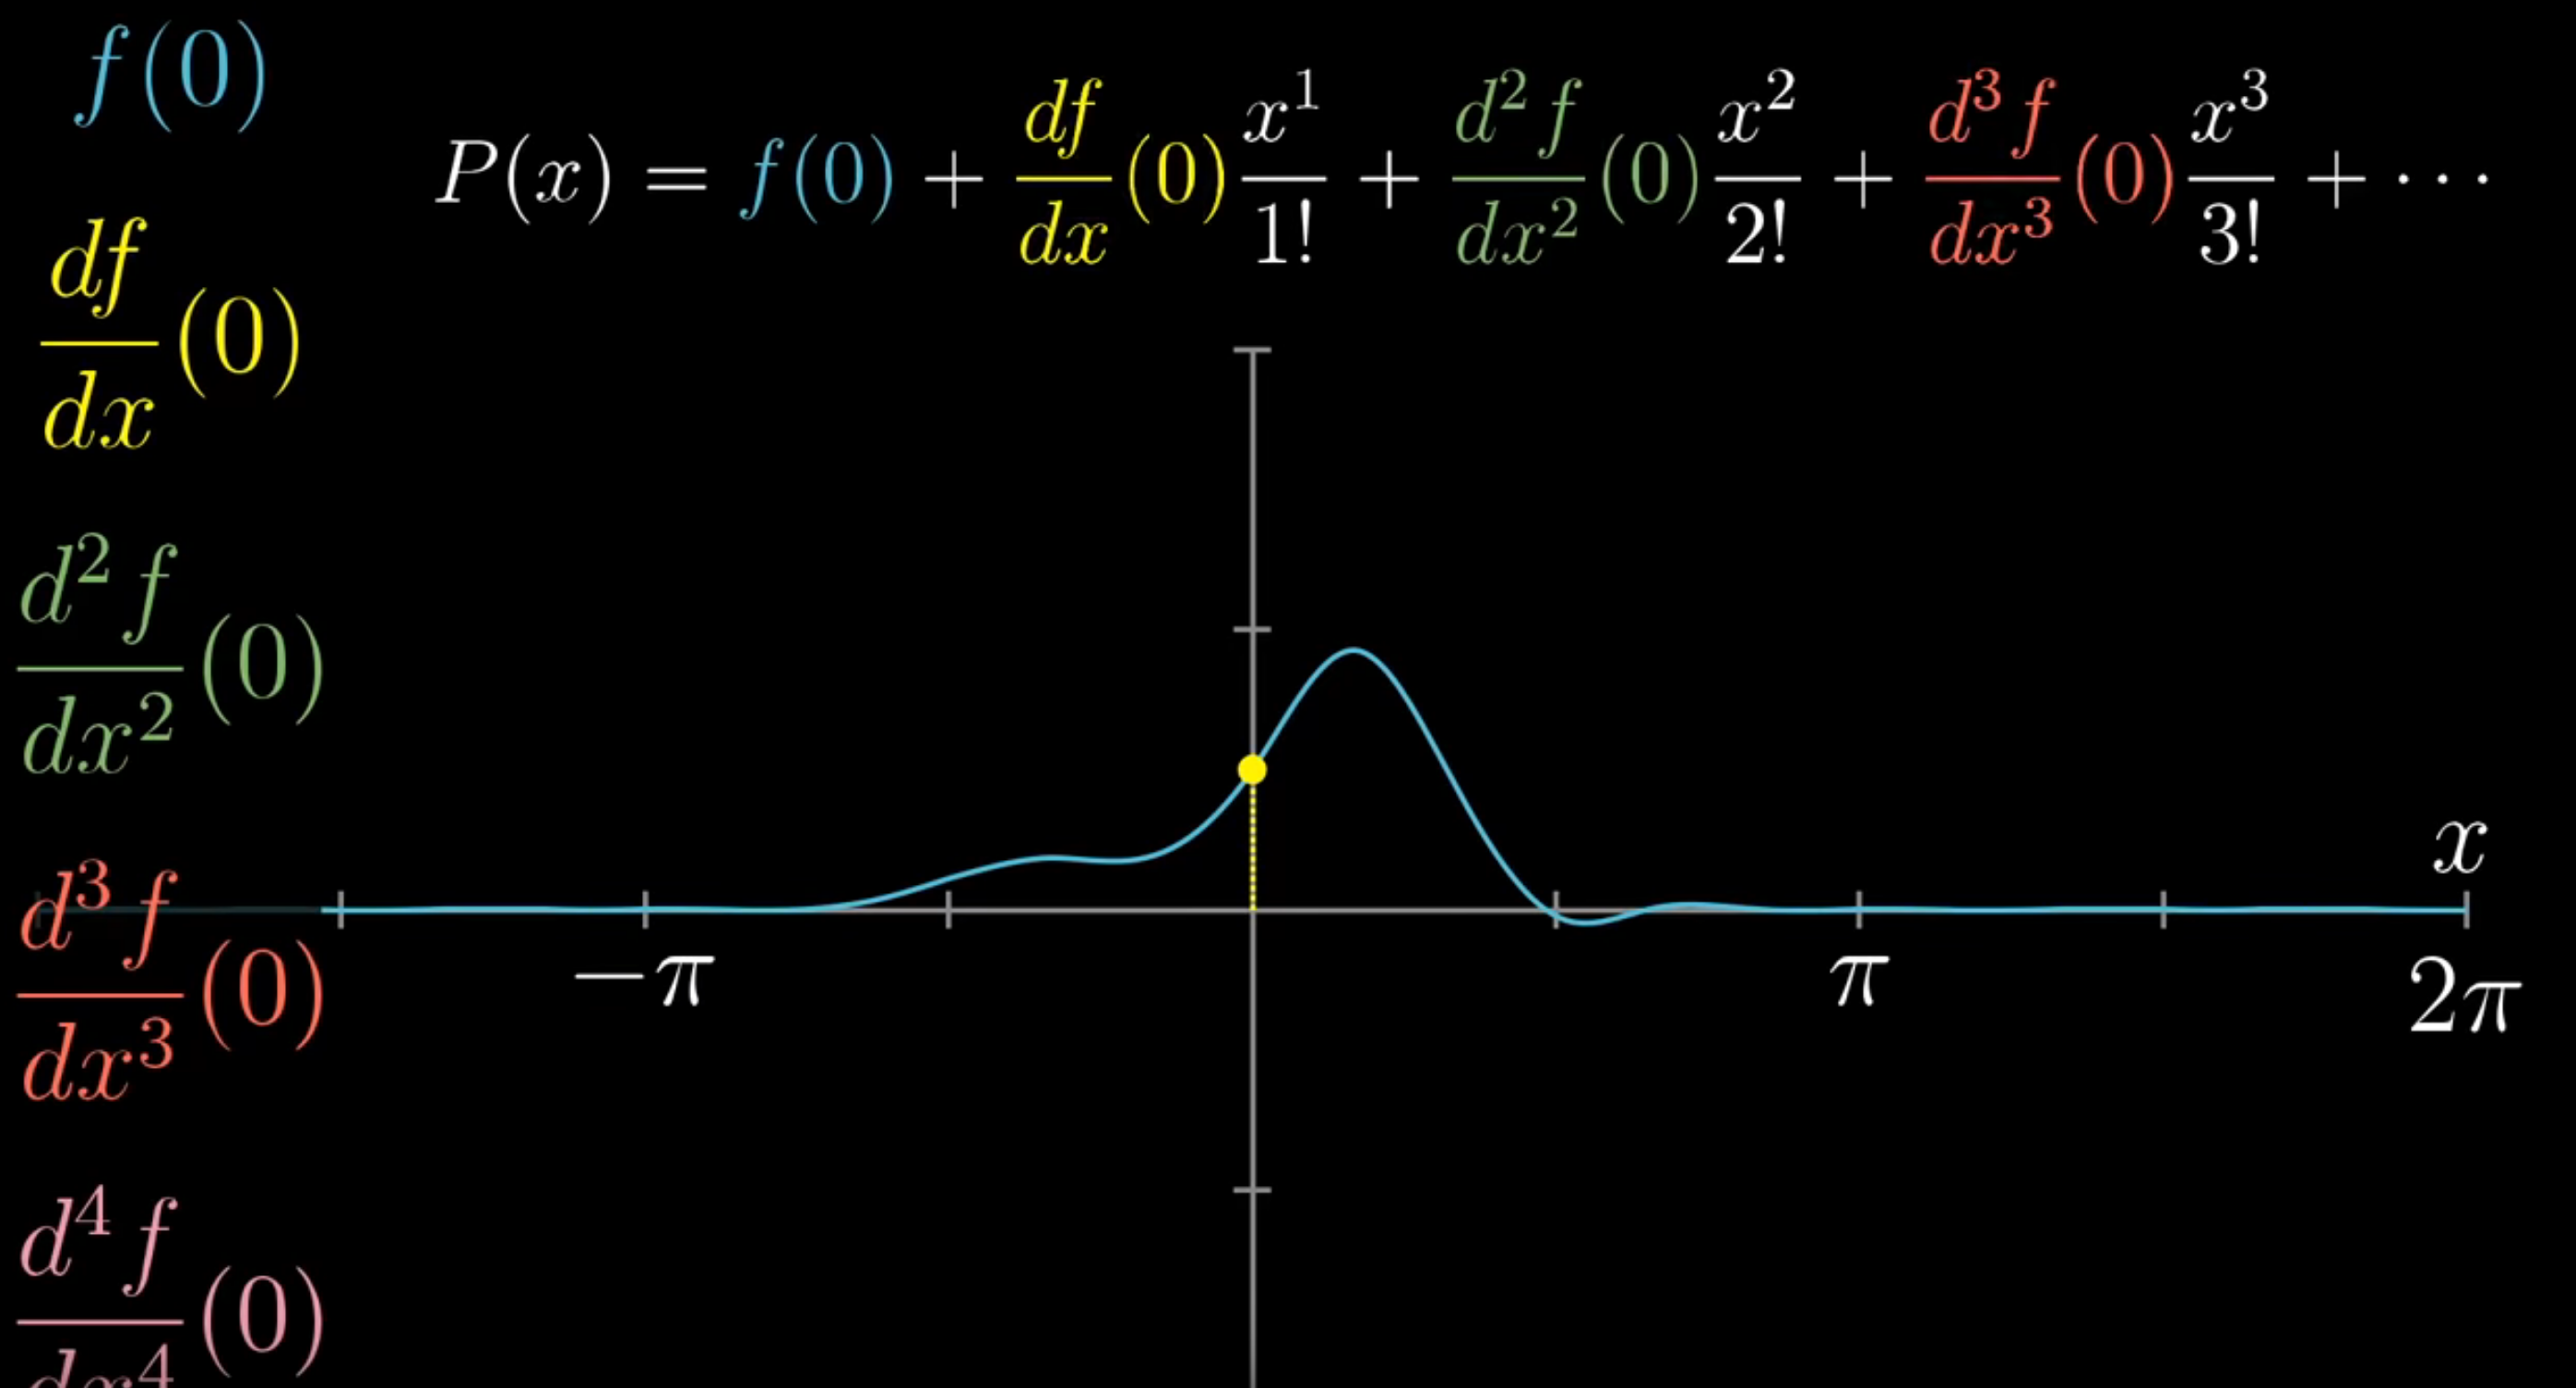
\includegraphics[width=\textwidth]{figs/taylor-polynomial.png}
		\end{figure}
	}
	\mode<handout>{
		\vspace{5cm}
	}
\end{frame}


%------------------------------------------------
\begin{frame}
	\frametitle{Taylor series: Generalization}
	\mode<beamer>{
		\begin{figure}[ht]
			\centering
			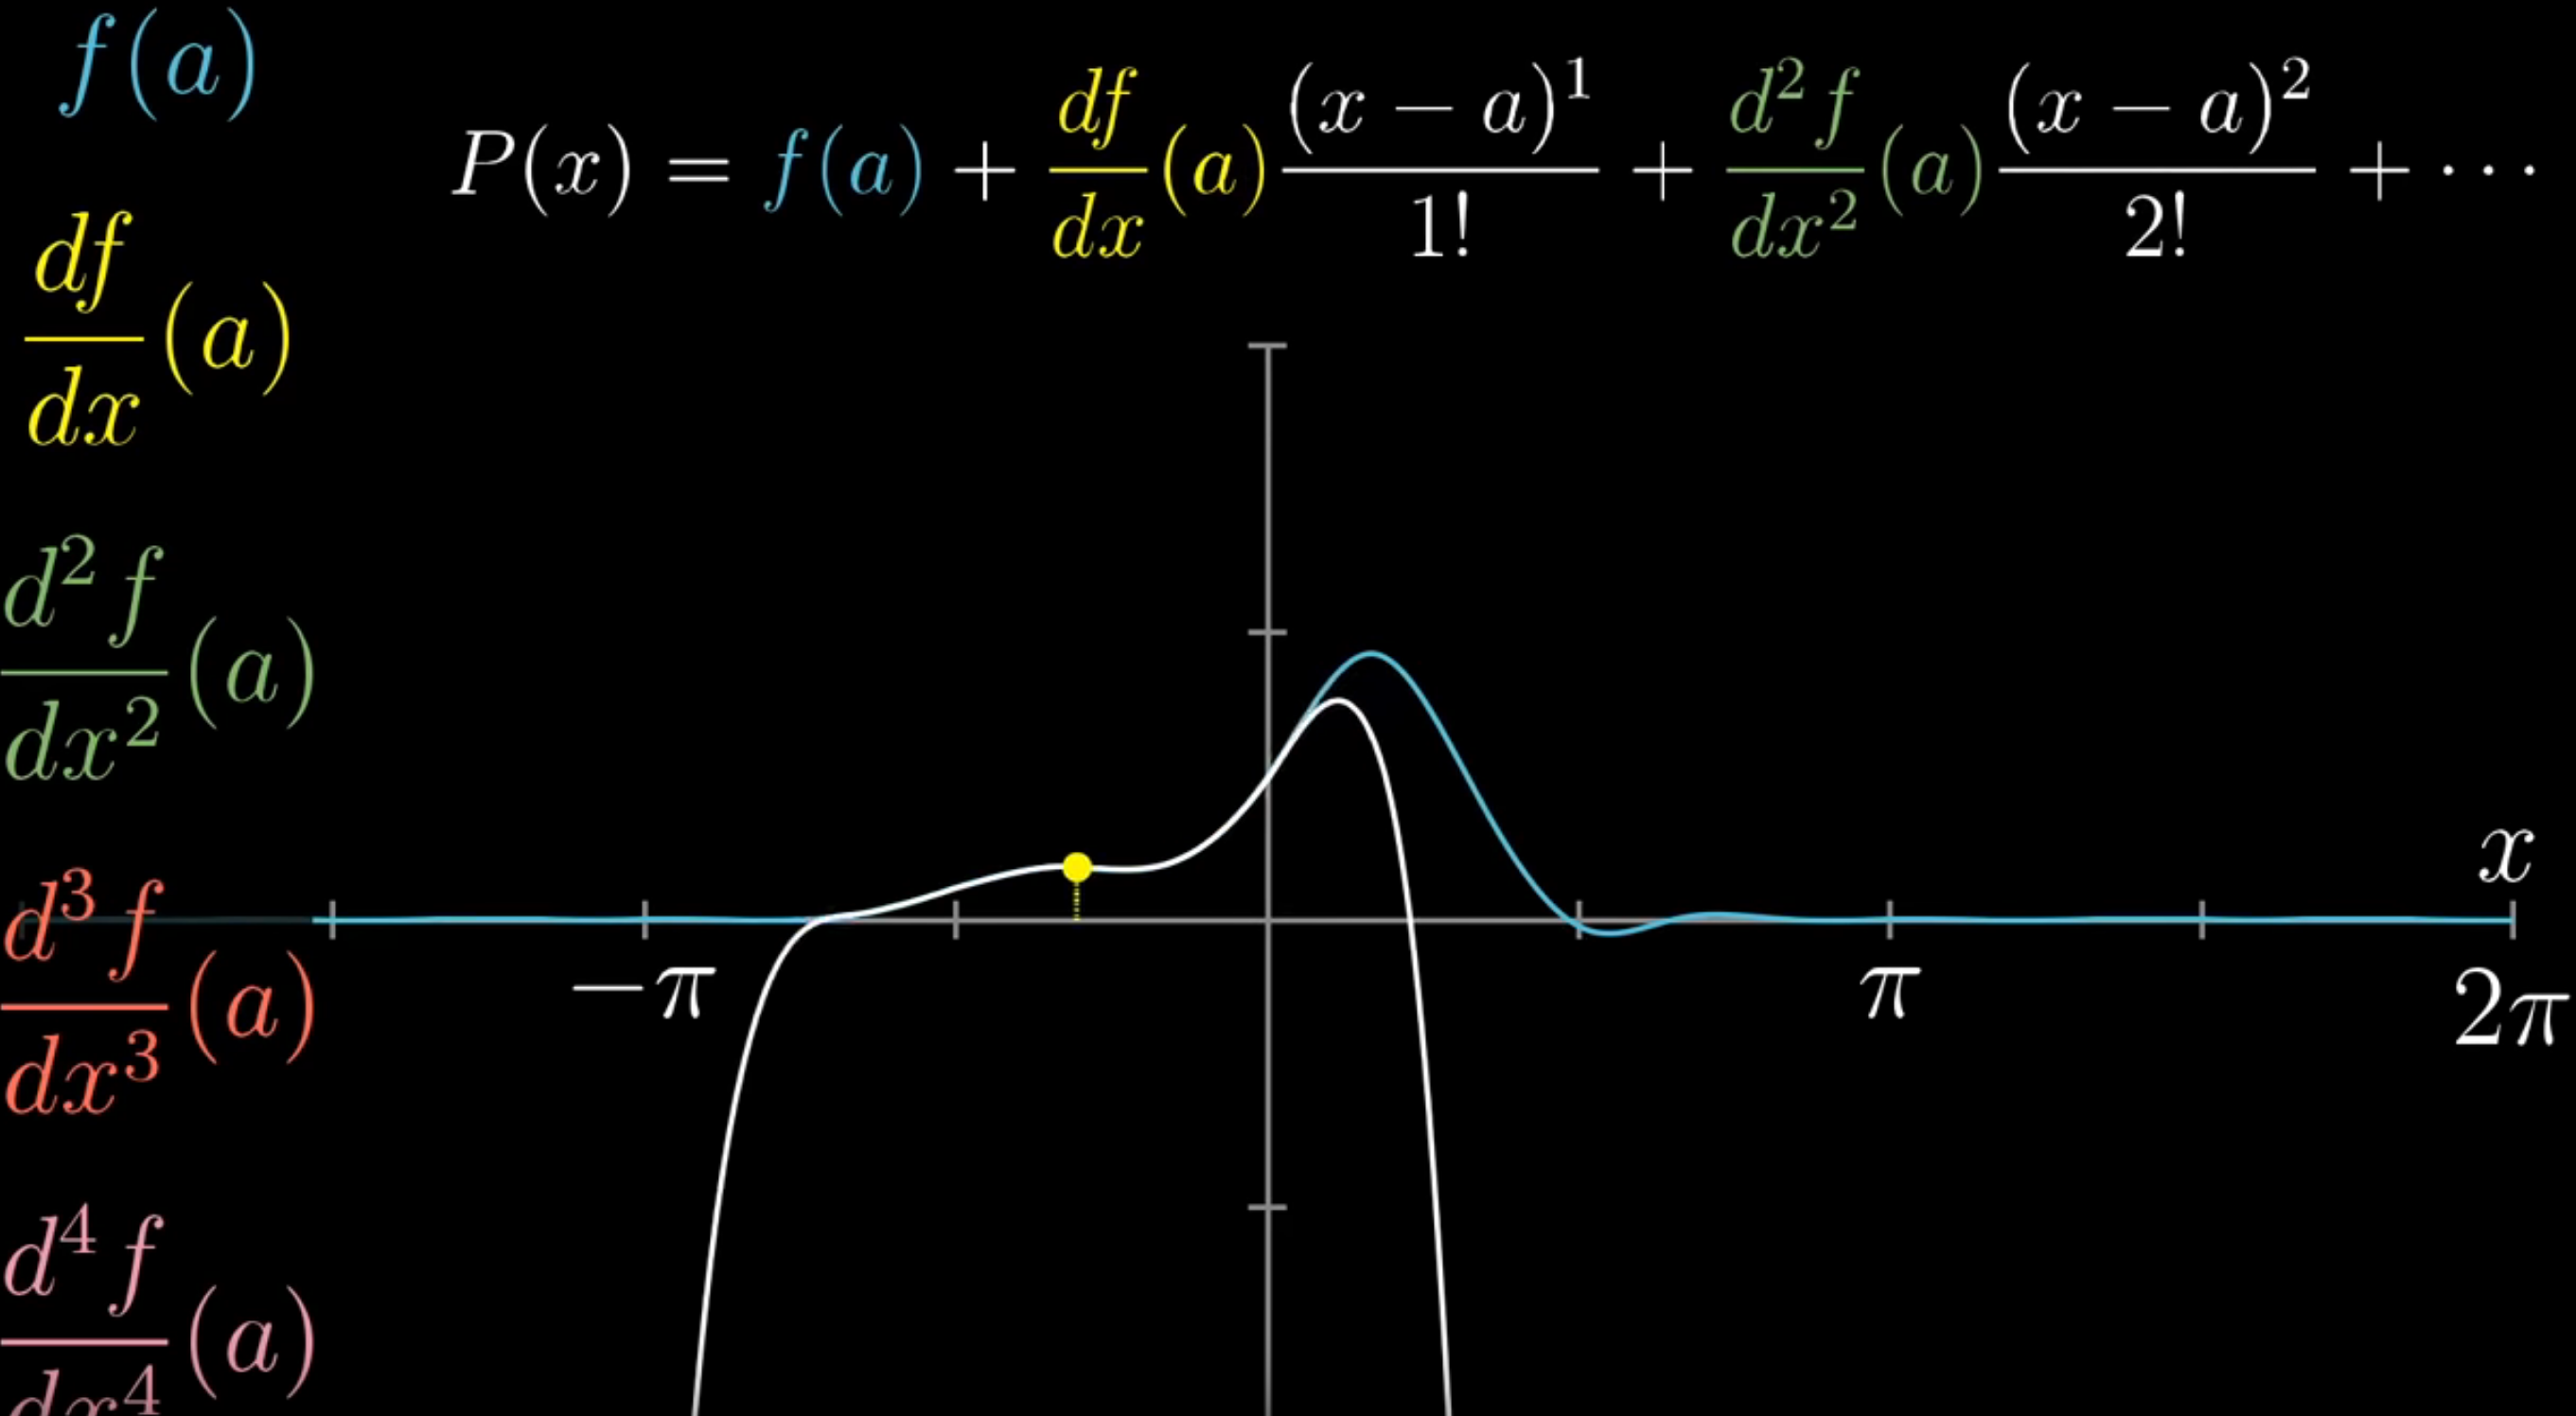
\includegraphics[width=\textwidth]{figs/general-taylor-series.png}
		\end{figure}
	}
	\mode<handout>{
		\vspace{5cm}
	}
\end{frame}


%------------------------------------------------
\begin{frame}
	\frametitle{Taylor series: Two variables}
	The Taylor series of $f$ expanded about $(x,y)=(a,b)$ is:	
	\mode<beamer>{
	\begin{equation*}
		\begin{split}
		(x,y)=f(a,b)+\frac{\partial f}{\partial x}(a,b)\cdot (x-a)+\frac{\partial f}{\partial y}(a,b)\cdot(y-b) \\
		+\frac{1}{2!}[\frac{\partial^2 f}{\partial x^2}(a,b)\cdot (x-a)^2\\ 
		+ 2 \frac{\partial^2 f}{\partial xy}(a,b)\cdot (x-a)(y-b)+\\ \frac{\partial^2 f}{\partial y^2}(a,b)\cdot (y-b)^2]+\cdots
		\end{split}
	\end{equation*}
	}
	\mode<handout>{
		\vspace{5cm}
	}
\end{frame}



\section{Newton Raphson}
%------------------------------------------------
\begin{frame}
	\frametitle{Newton Raphson}
 Assuming $r$ is a root of $f$ and that f is continuously differentiable in the
	vicinity of $r$ with $f^\prime (r) \ne 0$, then a sequence $(x_n)$ that converges to $r$ for $n \rightarrow \infty$ can be found using the Taylor expansion of $f$:
	\mode<beamer>{
		\begin{align*}
			f(r) & =  f(x_n + \varepsilon_n) = f(x_n) + f^\prime(x_n)\varepsilon_n + \frac{f^{\prime\prime}(x_n)}{2!}\varepsilon_n^2 \dots \\
			\varepsilon_n & \approx - \frac{f(x_n)}{f^\prime(x_n)} \\
			r = x_n + \varepsilon_n & \approx x_n - \frac{f(x_n)}{f^\prime(x_n)}
		\end{align*}
		in other words $ x_n - \frac{f(x_n)}{f^\prime(x_n)}$ is the next iteration of $r$, and hence we write:
	\begin{equation*}
	x_{n+1} = x_n - \frac{f(x_n)}{f^\prime(x_n)}
	\end{equation*} 
	}
	\mode<handout>{
		\vspace{5cm}
	}
\end{frame}
\note{
		We wish to find roots of $f(x)$ using a converging sequence $(x_n)$. But we want to do it faster.
		
	Newton's original method (1685) was purely algebraic, which he applied only to	polynomials and used a sequence of polynomials instead of successive approximations $x_n$.
	
	Raphson's simplified version (1690) was also only algebraic and he applied it only to polynomials but used $x_n$ approximations. 
	
	Simpson gave the form used today 50 years later (1740), along with other important results in the same paper.}


%------------------------------------------------
\begin{frame}
	\frametitle{Newton-Raphson graphical expression}
	\mode<beamer>{
		\begin{figure}[ht]
			\centering
			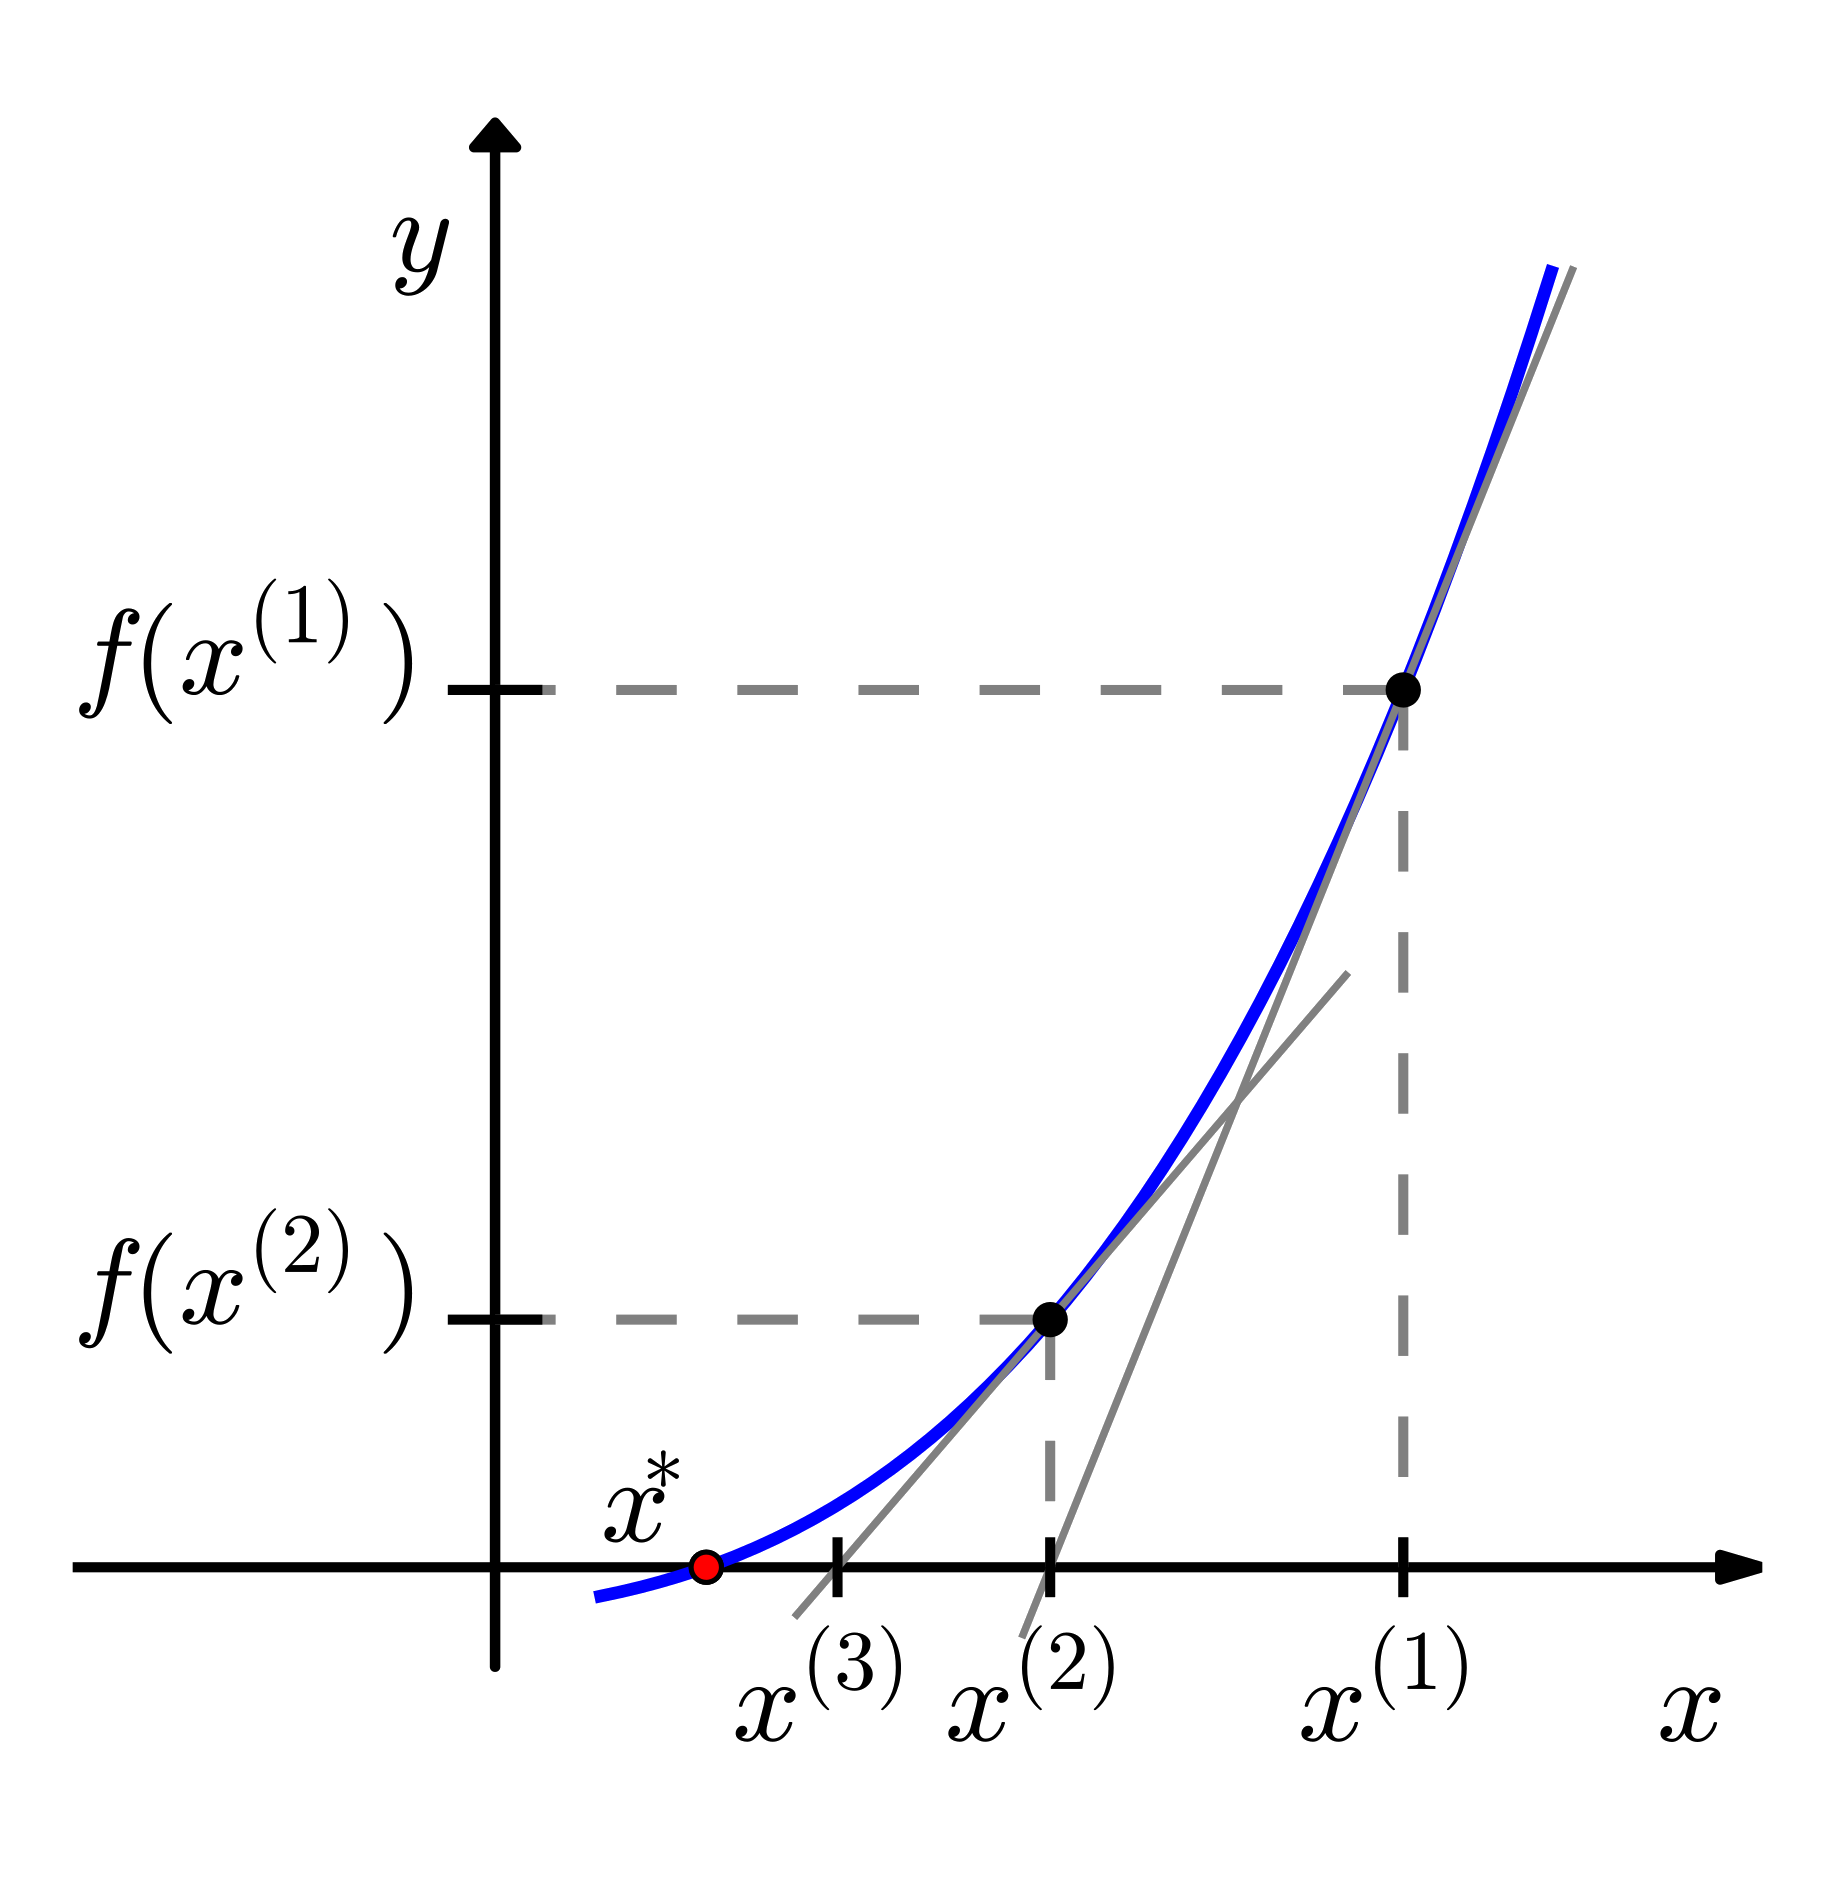
\includegraphics[width=0.65\textwidth]{figs/newton.png}
		\end{figure}
	}
	\mode<handout>{
		\vspace{5cm}
	}
\end{frame}

%------------------------------------------------
\begin{frame}
	\frametitle{Newton-Raphson failure}
	\begin{figure}[ht]
		\centering
		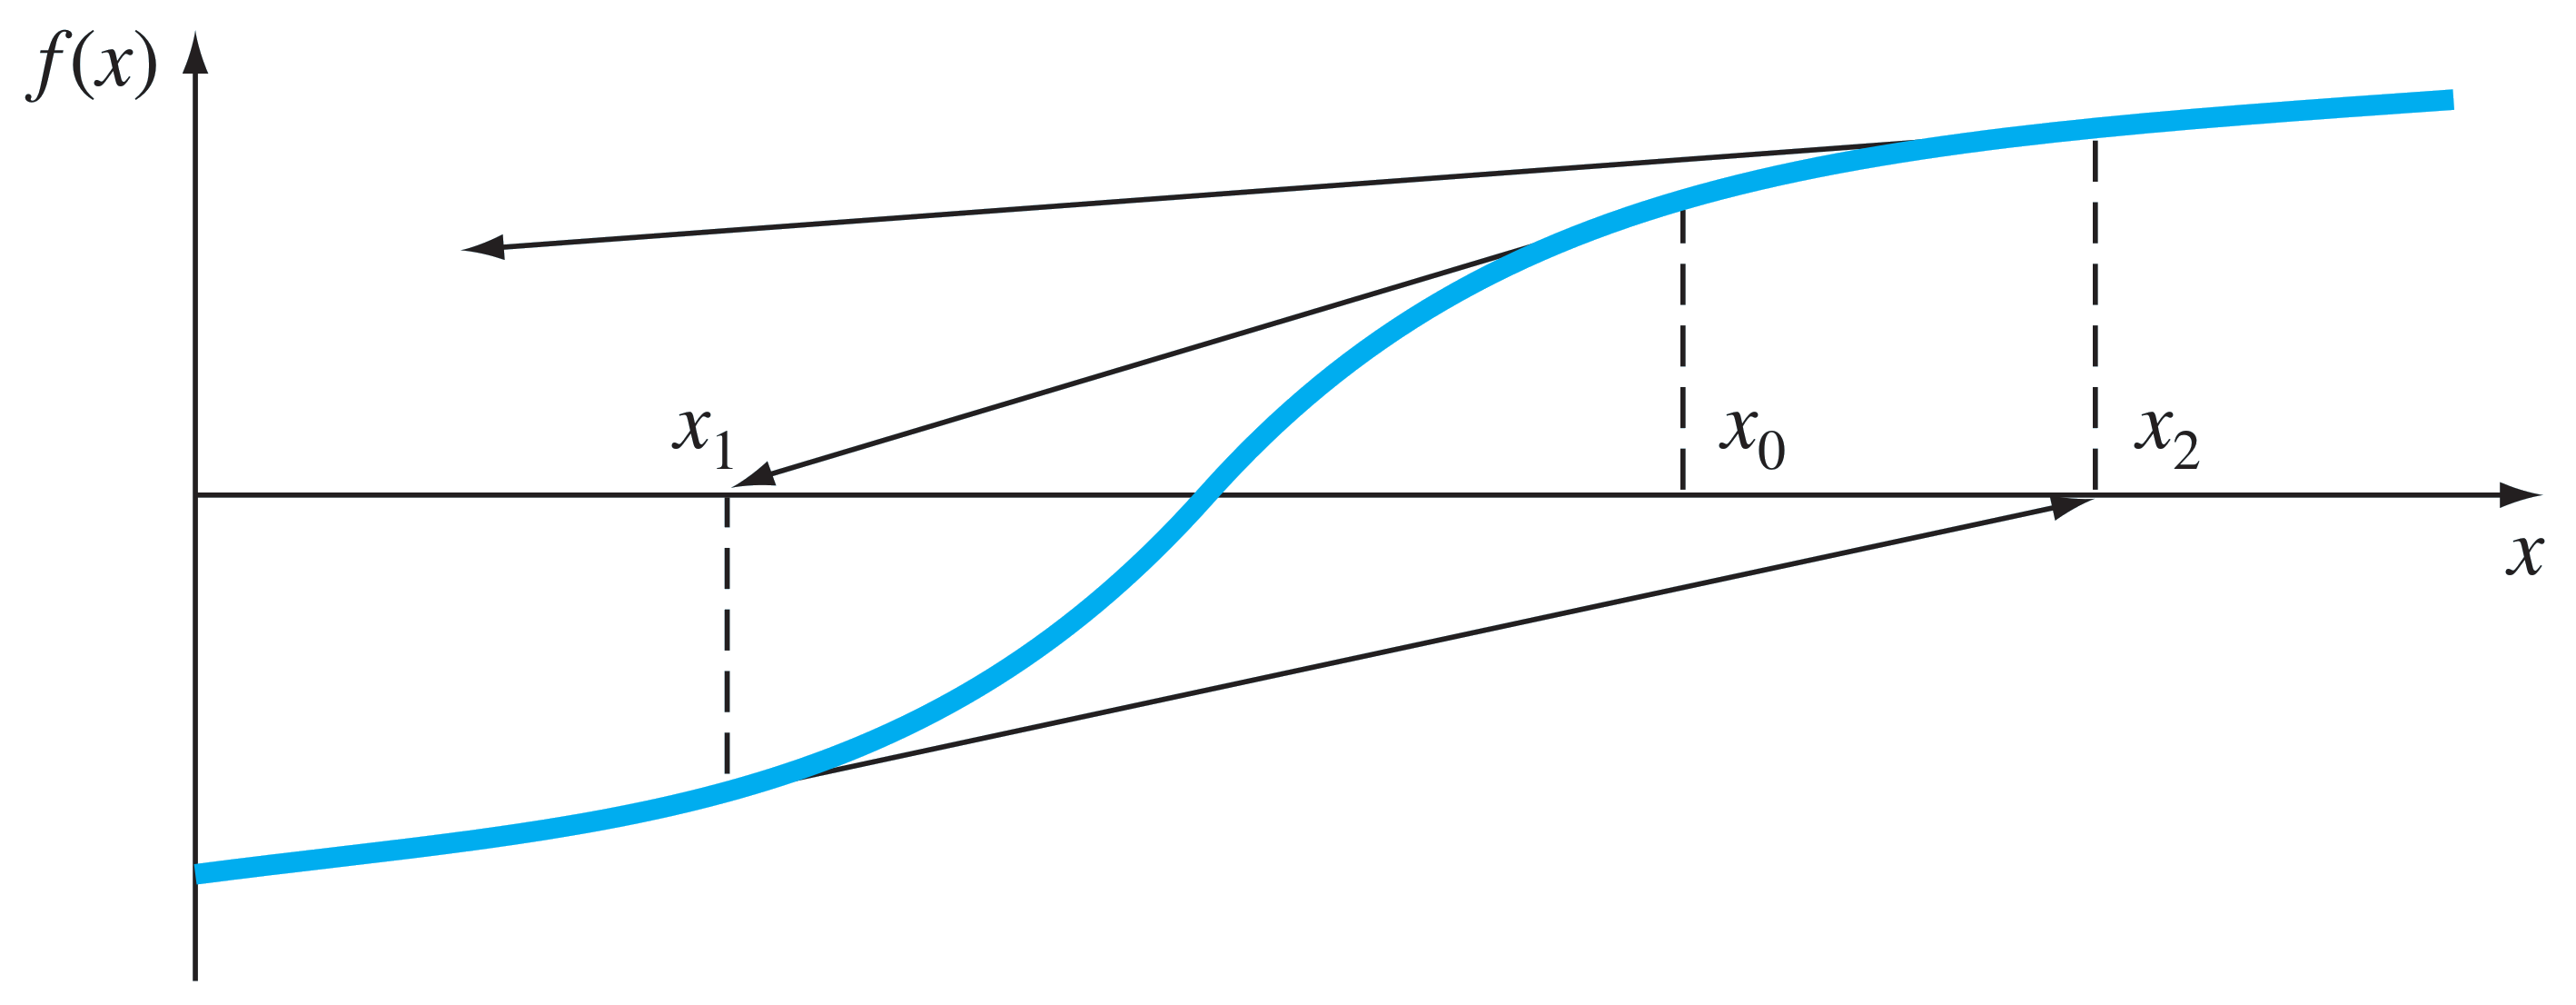
\includegraphics[width=\textwidth]{figs/nr-1.png}
	\end{figure}
\end{frame}


%------------------------------------------------
\begin{frame}
	\frametitle{Newton-Raphson failure}
	\begin{figure}[ht]
		\centering
		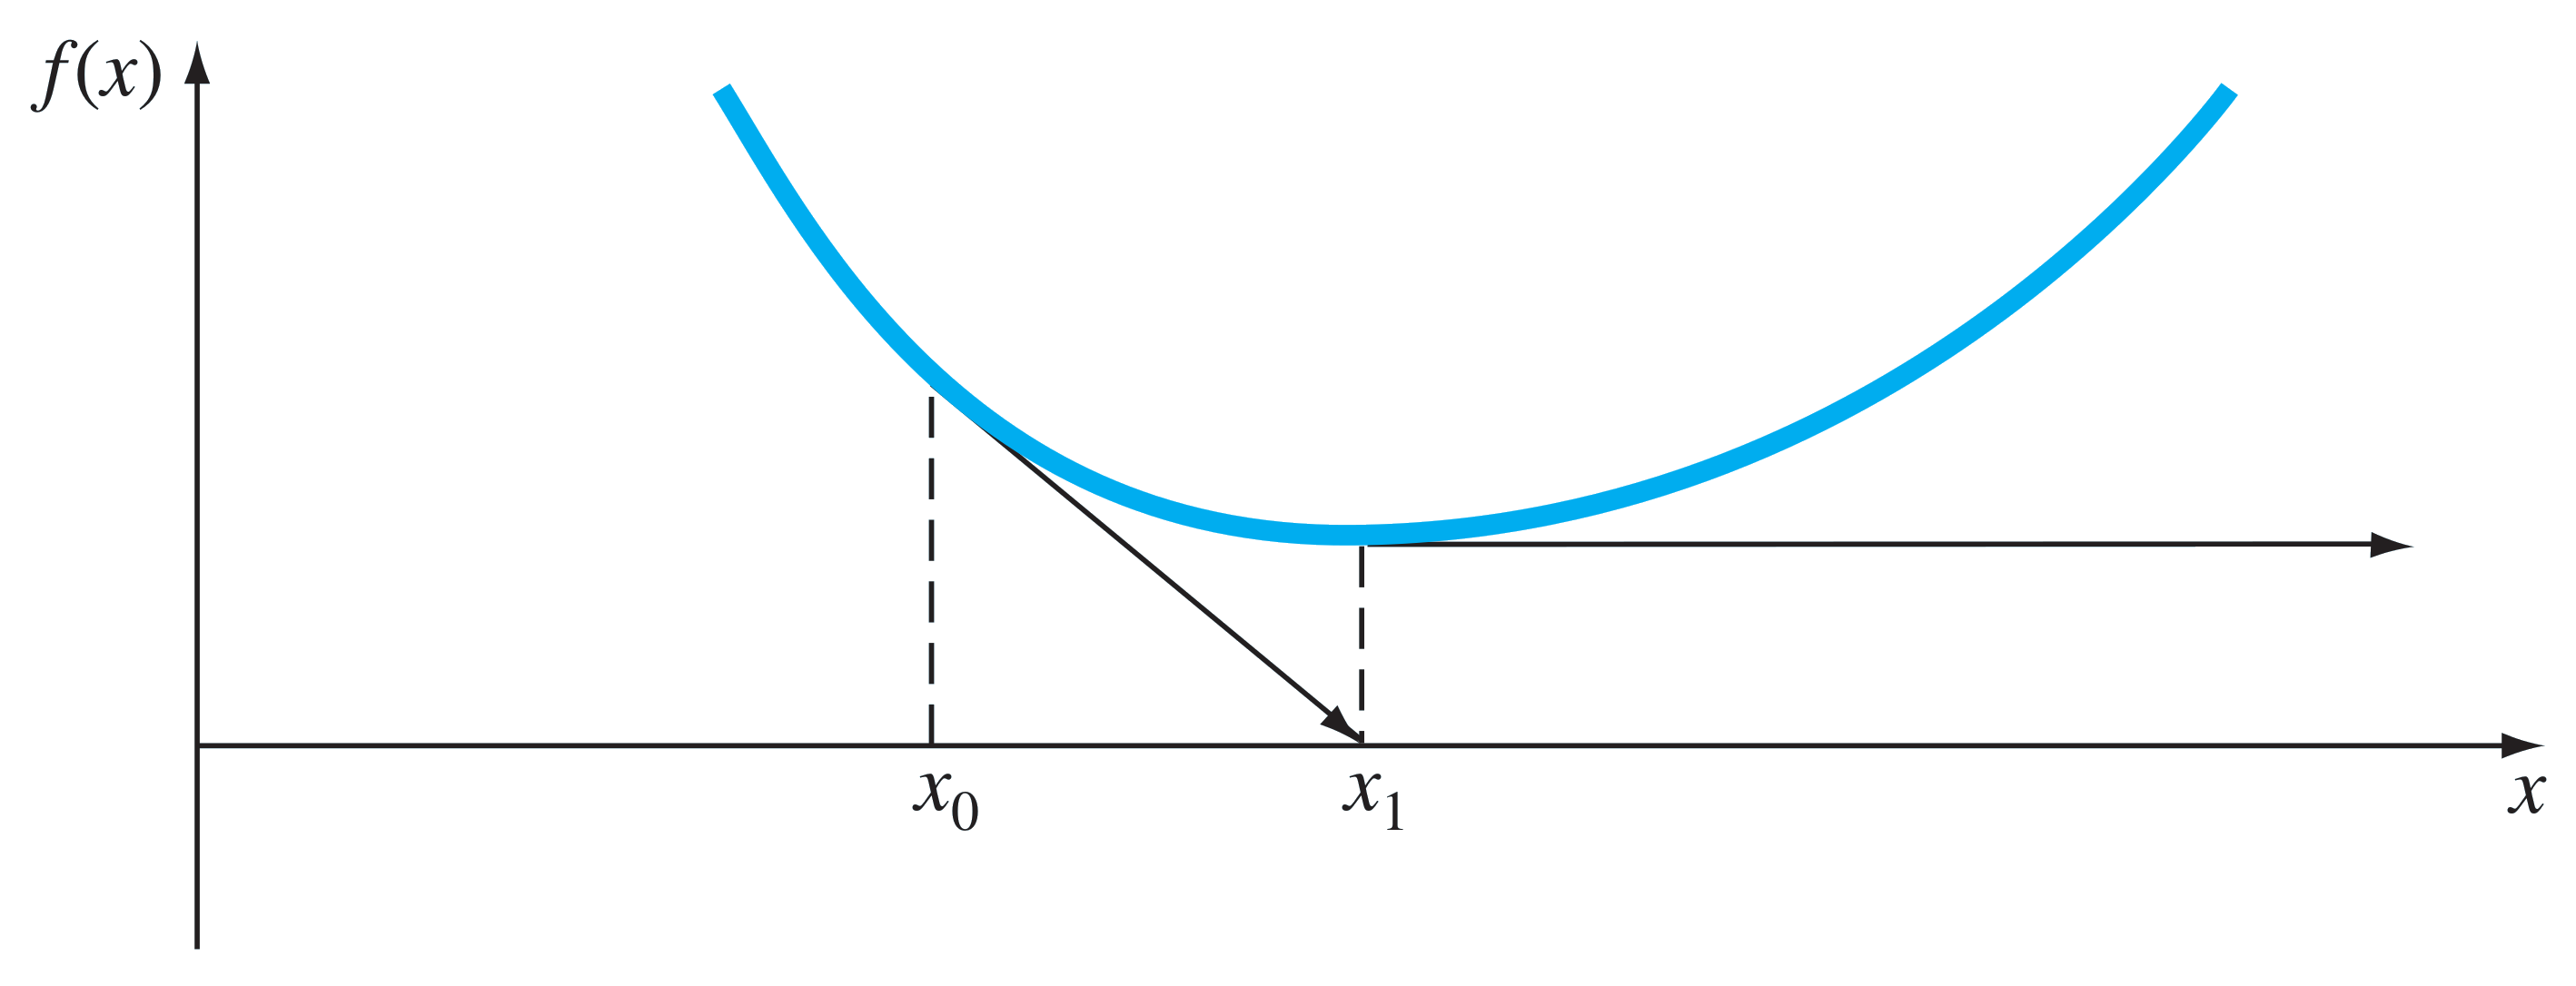
\includegraphics[width=\textwidth]{figs/nr-2.png}
	\end{figure}
\end{frame}

%------------------------------------------------
\begin{frame}
	\frametitle{Newton-Raphson failure}
	\begin{figure}[ht]
		\centering
		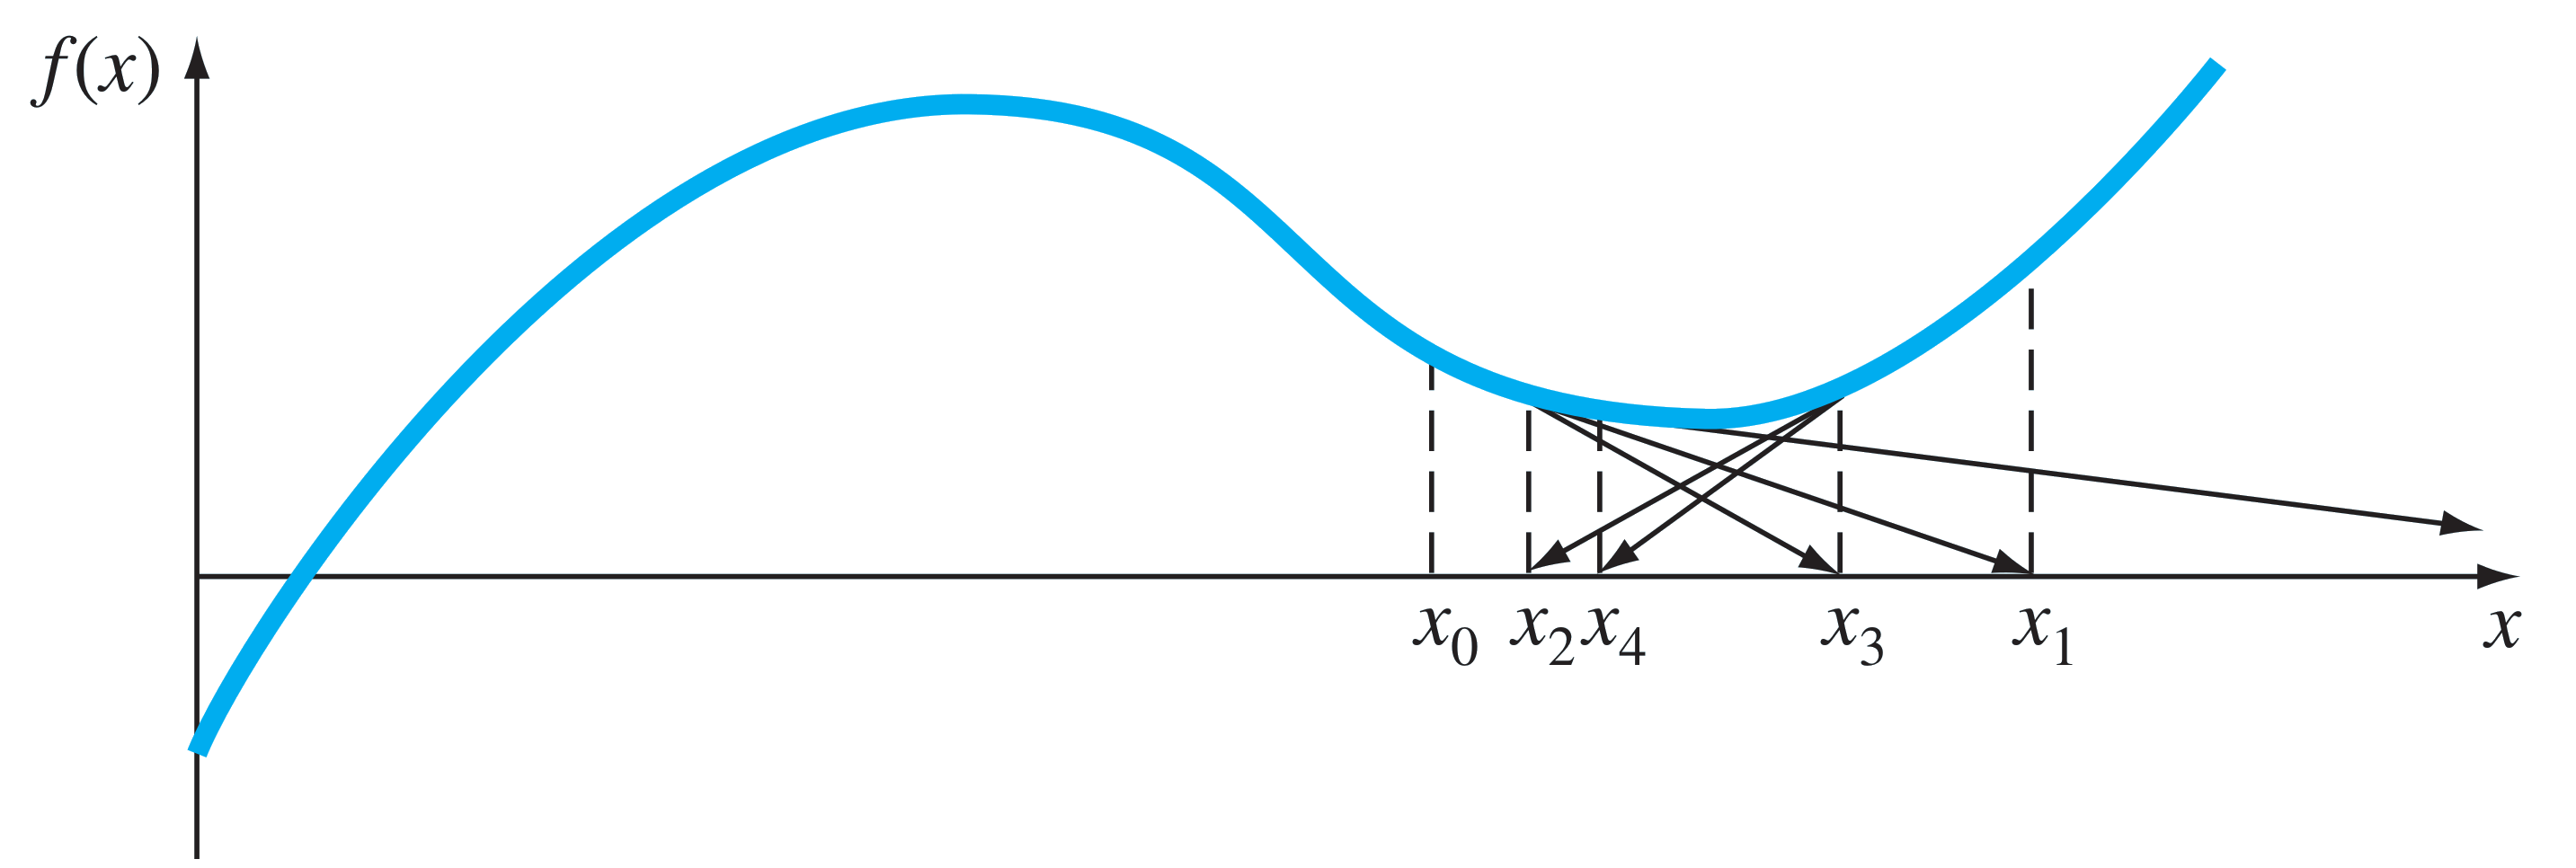
\includegraphics[width=\textwidth]{figs/nr-3.png}
	\end{figure}
\end{frame}

\end{document}
